\documentclass[conference]{IEEEtran}
\usepackage{times}

\usepackage{amsmath, amsfonts, amsbsy, amssymb, amsthm}

\let\labelindent\relax
\usepackage{mathtools}
\usepackage[table,xcdraw]{xcolor}
\usepackage{enumitem}
% \usepackage[numbers,compress]{natbib}
\usepackage{multicol}
\usepackage[bookmarks=true]{hyperref}
\usepackage{adjustbox}
\usepackage{graphicx, booktabs}
\usepackage{float}
\usepackage[english]{babel}

\usepackage[caption=false,font=footnotesize]{subfig}
\usepackage{multirow}
\usepackage{siunitx}
\usepackage{tikz}
\usepackage[dvipsnames]{xcolor}

\usetikzlibrary{arrows.meta,positioning,calc,fit,backgrounds}
\newcommand{\ustag}[1]{{\color{black!55}\scriptsize #1}}
\newcommand{\how}[1]{{\color{black!55}\itshape\footnotesize #1}}
\newcommand{\howtag}[1]{{\color{black!60}\itshape\tiny #1}}

\newtheorem*{problem}{Problem}
\newtheorem{remark}{Remark}
\newtheorem{assumption}{Assumption}
\newtheorem{proposition}{Proposition}
\newtheorem{corollary}{Corollary}
\newtheorem{lemma}{Lemma}
\newtheorem{theorem}{Theorem}
\newtheorem{property}{Property}

\newcommand{\mm}[1]{{\color{red}{{#1}}}}
\newcommand{\cl}[1]{{\color{Red}{{#1}}}}
\newcommand{\ls}[1]{{\color{blue}{{#1}}}}

\newenvironment{proofsketch}{%
  \renewcommand{\proofname}{Sketch of Proof}\proof}{\endproof}



\begin{document}
\title{Real-Time Ergodic Control via Curl-Augmented Flow Matching with MPPI}

\author{Author Names Omitted for Anonymous Review.}
% \author{Mattia Mantovani, Mattia Catellani and Lorenzo Sabattini}
\maketitle

\begin{abstract}
Ergodic coverage seeks robot trajectories whose long-term state visitation matches a target spatial distribution. Existing approaches face a trade-off between feedback controllers that rely on trajectory history and optimization-based methods that achieve high-quality coverage but are not suitable for real-time replanning.
%
We propose a sampling-based ergodic controller that integrates flow-matching objectives directly into Model Predictive Path Integral (MPPI) control. Our key idea is to shape the rollout-induced ensemble distribution so that its predicted visitation statistics follow a prescribed probability flow consistent with the target density.
%
We construct a reference flow using Stein variational gradient dynamics and introduce a curl-augmented component that improves mixing while preserving the target invariant distribution. \cl{Long-run coverage is driven by feedback from a bounded, fixed-size fading memory of recent visitation, so the controller carries a constant-memory history rather than the growing trajectory history of classical spectral methods.} Flow alignment is implemented as an additive rollout cost, allowing ergodic objectives and task-specific constraints to be handled uniformly within MPPI's importance sampling framework.
%
The resulting model-independent controller provides a real-time, closed-loop approach for constrained \cl{ergodic coverage with constant memory}. Extensive simulations and software-in-the-loop experiments demonstrate efficient ergodic exploration with continuous online replanning.
\end{abstract}

\IEEEpeerreviewmaketitle

\section{Introduction}
\cl{Can we achieve ergodic coverage with a real-time, constant-memory MPPI ergodic controller?}
Ergodic coverage refers to the generation of trajectories such that the asymptotic spatial distribution of state visitation aligns with a prescribed target distribution. This facilitates exploration that is proportional to the information density of the environment, as opposed to traditional waypoint-based navigation strategies. The ergodic coverage framework is particularly advantageous for active sensing problems that demand persistent spatial coverage, and it has demonstrated utility in domains such as multi-robot exploration, reinforcement learning, and embodied manipulation.

Classical ergodic control was formalized through spectral discrepancy metrics and feedback controllers that depend on trajectory history, notably Spectral Multiscale Coverage (SMC)~\cite{mathew2009spectral, mathew2011metrics}, and has supported applications ranging from multi-robot exploration~\cite{wittemyer2025, abraham2018decentralized, sartoretti2021spectral} to reinforcement learning~\cite{berrueta2024maximum}. A dominant modern line embeds ergodic objectives into finite-horizon trajectory optimization~\cite{miller2013trajectory, miller2016ergodic, ayvali2017ergodic}, including time-optimal~\cite{dong2023time, dong2023timeSAGE}, geometry-aware~\cite{xu2024measurepreservingflowsergodic}, and safety-constrained variants~\cite{lerch2023safety}. While effective, these approaches remain optimization-heavy and are not naturally suited for real-time closed-loop replanning. Complementary PDE-based methods such as HEDAC~\cite{ivic2017hedac, ivic2019spraying, ivic2022constrained} avoid explicit discrepancy metrics but require online PDE solves, which can be computationally demanding and difficult to integrate with complex constraints. Recent advances have also explored kernel-based accelerations~\cite{hughes2025ergodic, sun2024fast} and sampling-based formulations, including Stein variational methods~\cite{lee2024stein} and flow-matching approaches~\cite{lipman2022flow, sun2025flow}, which reinterpret ergodic coverage as a distribution shaping problem.
\begin{figure}[tb]
    \centering
    \includegraphics[width=1\linewidth]{pictures/overview.png}
    \caption{The figure illustrates a representative software-in-the-loop (SITL) run, showing the proposed controller operating in simulation.}
    \label{fig:overview}
\end{figure}
Despite this progress, achieving ergodic exploration that is simultaneously closed-loop, real-time capable, and constraint-aware remains challenging. Optimization-based methods can incorporate constraints but require repeated global solves, limiting responsiveness to disturbances and dynamic environments. Conversely, reactive controllers provide real-time feedback but often lack the long-horizon reasoning needed to match complex spatial distributions.

In this work, we address this gap by casting ergodic control as \emph{distribution shaping of the rollout-induced ensemble} within Model Predictive Path Integral (MPPI) control. Rather than explicitly minimizing a global ergodic metric or solving a trajectory optimization problem, we shape the distribution of sampled rollouts so that their predicted visitation statistics follow a prescribed probability flow consistent with the target density. This preserves MPPI's key advantages: real-time replanning, model-agnostic operation, and seamless integration of constraints through cost design.

We construct the target flow using Stein variational gradient dynamics and augment it with a nonreversible curl component that improves mixing in multi-modal distributions while preserving the target invariant density. \cl{To obtain long-run ergodicity, and not merely within-horizon spread, the flow additionally receives feedback from a bounded fading memory of recently executed positions, weighted by the local over-coverage relative to the target and evaluated over a bank of spatial scales.} The desired flow is incorporated as an additive rollout cost, allowing MPPI's importance sampling mechanism to implicitly bias trajectories toward ergodic behavior. This avoids backpropagation through the dynamics and does not require model linearization or offline optimization. A rollout-based sensitivity estimator, equivalent to a score-function estimator, can be used to interpret the induced update direction, but the method itself operates entirely through cost shaping.

The resulting controller provides a real-time, closed-loop, and \cl{constant-memory (bounded fading-memory)} approach to ergodic coverage, capable of handling constraints and disturbances within a unified sampling-based framework. The main contributions of this work are:
\begin{itemize}[leftmargin=*]
    \item We formulate real-time ergodic exploration as distribution shaping of the rollout-induced MPPI ensemble.
    \item We introduce a curl-augmented reference flow that improves inter-mode mixing while preserving the target density.
    \item \cl{We drive long-run coverage with a constant-size fading-memory feedback whose repulsion is weighted by the online relative over-coverage across a bank of spatial scales, a closed-form surrogate for the multiscale ergodic-metric gradient, governed by three interpretable parameters.}
    \item We embed flow matching as an additive rollout cost in MPPI, enabling unified handling of ergodic objectives and constraints.
    \item We provide a conditional asymptotic analysis relating the stationary mismatch of the closed-loop visitation law to the resulting ergodic error, \cl{for the memory-augmented closed-loop Markov chain}.
    \item We validate the proposed method through extensive simulations and software-in-the-loop experiments.
\end{itemize}

\section{Background \& Notation}
\label{sec:notation}

Let $\Omega\subset\mathbb{R}^{d_s}$ be a bounded workspace, and let $p^\star(\mathbf z)$ be a normalized target density on $\Omega$.
We use a receding-horizon controller with a prediction horizon $T$ and horizon index $k\in\{0,\dots,T\}$.
To avoid ambiguity, we distinguish: (i) horizon time $k$ within a single planning call, (ii) physical replanning time $t$ (advance $t\!\to\!t+\Delta t$ after executing the first control), and (iii) an auxiliary flow time $s$ for internal distribution-shaping updates at fixed $t$.
Unless stated otherwise, we consider one planning call at fixed $t$ and perform a single flow update; thus, the dependence on $s$ is omitted.
Uppercase symbols (e.g., $\mathbf{X}_{t,k},\mathbf{U}_{t,k}$) denote random variables, and lowercase symbols (e.g., $\mathbf{x}_{t,k}^{(b)},\mathbf{u}_{t,k}^{(b)}$) denote realizations.

\subsection{Measure-Preserving Definition of Ergodicity}\label{sec:ergodicity}
%
From a dynamical-systems perspective, a system is ergodic if time averages along its trajectories equal spatial averages with respect to an invariant probability measure.
For an executed trajectory $\psi:[0,L]\!\to\!\Omega$ of length $L$, define the empirical visitation distribution
%
\begin{equation}
    c_{\psi,L}(\mathbf{z})=\frac{1}{L}\int_0^L \delta(\mathbf{z}-\psi(\tau))\,d\tau,
\end{equation}
%
where \(\delta(\cdot)\) is the Dirac delta.
Ergodicity with respect to a target density $p^\star$ can be quantified by comparing the time-averaged and measure-averaged occupancy of local regions. One such discrepancy metric is
\begin{equation}\label{eq:ergodic_metric}
\begin{aligned}
    \mathcal{E}(\psi, p^\star) = \int_0^R\! \int_{\Omega} \Bigg[ \frac{1}{L} &\int_0^L \mathbf{1}_{(\mathbf{z}, r)}(\psi(\tau)) \, d\tau - \\
    &\int_{\Omega} \mathbf{1}_{(\mathbf{z}, r)}(\mathbf y) \, p^\star(\mathbf y) \, d\mathbf y \Bigg]^2 d\mathbf{z} \, dr,
\end{aligned}
\end{equation}
where $\mathbf{1}_{(\mathbf z,r)}$ denotes the indicator function of the ball
$B(\mathbf z,r)=\{\mathbf y\in\Omega:\|\mathbf y-\mathbf z\|\le r\}$,
and $R>0$ is the maximum spatial scale considered by the metric.
Thus, the integral over $r\in[0,R]$ compares occupancy statistics across multiple spatial scales, from local regions for small $r$ to coarser workspace-level regions for larger $r$.
This metric measures how closely the fraction of \emph{executed time} spent in regions of varying scale matches the probability mass assigned by $p^\star$.

A closed-loop system is ergodic with respect to $p^\star$ if, for any initial condition,
\begin{equation}
    \lim_{L\to\infty}\mathcal{E}(\psi, p^\star)=0,
\end{equation}
i.e., long-run visitation statistics along the executed trajectory converge to the target measure.

\subsection{Model Predictive Path Integral (MPPI) Control}\label{sec:mppi}
We consider stochastic optimal control problems in which the system evolves as an It\^o diffusion,
\begin{equation}\label{eq:sde}
    d\mathbf{x}_t = \mathbf{f}(\mathbf{x}_t,\mathbf{u}_t,t)\,dt + \mathbf{B}(\mathbf{x}_t,t)\,d\mathbf{w}_t,
\end{equation}
with state $\mathbf{x}_t\in\mathbb{R}^d$, control $\mathbf{u}_t\in\mathbb{R}^m$, and Wiener noise $\mathbf{w}_t$. The objective is to minimize the expected cumulative cost
\begin{equation}\label{eq:optimal_input}
    \mathbb{E}\left[\Phi(\mathbf{x}_{t_0+T\Delta t}) + \int_{t_0}^{t_0+T\Delta t} \mathcal{L}(\mathbf{x}_t,\mathbf{u}_t,t)\,dt\right],
\end{equation}
where \(\Phi(\cdot)\) and \(\mathcal L(\cdot)\) are the terminal and running stage costs respectively.
Path-integral (PI) control applies an exponential transformation that expresses the solution as an expectation over noise-perturbed trajectories, motivating sampling-based approximations.

MPPI implements this idea in a receding-horizon fashion via Monte Carlo rollouts. At a given physical time $t$, MPPI maintains a nominal control sequence over the horizon,
\(
\boldsymbol\mu_t \;\coloneqq\; [\boldsymbol\mu_{t,0},\dots,\boldsymbol\mu_{t,T-1}] \in \mathbb{R}^{mT}.
\)
Drawing $N$ i.i.d.\ realizations $\{\mathbf{u}^{(b)}\}_{b=1}^{N}$ yields $N$ rollouts, sampled with independent Gaussian perturbations at each horizon step,
\begin{equation}\label{eq:mppi_sampling}
    \mathbf{u}^{(b)}_{t,k} = \boldsymbol\mu_{t,k} + \boldsymbol\epsilon^{(b)}_{t,k},
    \qquad \boldsymbol\epsilon^{(b)}_{t,k} \sim \mathcal{N}(\mathbf 0,\boldsymbol\Sigma),
\end{equation}
where $\mathbf{u}^{(b)}_{t,k}$ denotes the $k$-th control of rollout $b$. Equivalently, the joint sampling density factorizes as
\begin{equation}\label{eq:control_dist_factorized}
p(\mathbf{u}\mid\boldsymbol\mu_t)
=
\prod_{k=0}^{T-1}\mathcal{N}\!\big(\mathbf{u}_k\mid\boldsymbol\mu_{t,k},\boldsymbol\Sigma\big),
\end{equation}
where $\mathbf{u}=[\mathbf{u}_0,\dots,\mathbf{u}_{T-1}]$ denotes a generic realization of the sampled control sequence. \cl{Collecting all sampled perturbations across the $N$ rollouts and $T$ horizon steps, we write}
\begin{equation}\label{eq:Xi_def}
\Xi_t \;\coloneqq\; \big\{\, \boldsymbol\epsilon^{(b)}_{t,k}
\;:\; b\in\{1,\dots,N\},\; k\in\{0,\dots,T-1\} \,\big\},
\end{equation}
\cl{the full collection of $NT$ Gaussian perturbations drawn at replanning time $t$,} a notation used throughout the closed-loop analysis of Sec.~\ref{sec:guarantees}.
Each rollout is propagated through the discretized dynamics, $\mathbf{x}^{(b)}_{t,k+1}=f_d(\mathbf{x}^{(b)}_{t,k},\mathbf{u}^{(b)}_{t,k})$ with $\mathbf{x}^{(b)}_{t,0}=\mathbf{x}_t$, and assigned the cumulative cost
\begin{equation}
    S^{(b)}(\mathbf{x}_t,\boldsymbol\mu_t,\Xi_t) := \Phi(\mathbf{x}_{t,T}^{(b)}) + \sum_{k=0}^{T-1} \mathcal L(\mathbf{x}_{t,k}^{(b)},\mathbf{u}_{t,k}^{(b)}).
\end{equation}
\mm{We write the bare symbol $S^{(b)}$ whenever the dependence on $(\mathbf{x}_t,\boldsymbol\mu_t,\Xi_t)$ is clear from context.} MPPI forms exponential importance weights
\begin{equation}\label{eq:mppi_weights}
    \tilde{w}^{(b)}
    =
    \exp\!\left(
        -\frac{1}{\lambda}\left(
            S^{(b)}+
            \lambda(1-\alpha)\sum_{k=0}^{T-1}
            \big(\mathbf u^{(b)}_{t,k}\big)^\top
            \boldsymbol\Sigma^{-1}\boldsymbol\mu_{t,k}
        \right)\!\!
    \right),
\end{equation}
where the normalized weights are $w^{(b)} = \tilde{w}^{(b)}\big/\!\sum_{j=1}^{N}\tilde{w}^{(j)}$ as in~\cite{williams2018MPPI}, $\lambda$ is the temperature, and $\alpha$ scales the control-effort term. \mm{Since $S^{(b)}$ depends on $(\mathbf{x}_t,\boldsymbol\mu_t,\Xi_t)$, so do the resulting weights $w^{(b)}$ and the updated nominal sequence below; we make this dependence explicit only where needed for the closed-loop analysis of Sec.~\ref{sec:guarantees}.} The nominal sequence is then updated by the weighted average
\begin{equation}\label{eq:mppi_update}
    \boldsymbol\mu^{+}_{t,k} = \boldsymbol\mu_{t,k} + \sum_{b=1}^{N} w^{(b)}\,\boldsymbol\epsilon^{(b)}_{t,k},
    \qquad k=0,\dots,T-1.
\end{equation}
Following a receding horizon approach, only the first control $\boldsymbol\mu^{+}_{t,0}$ is executed before replanning at $t+\Delta t$.

\paragraph*{Closed-loop interpretation}
Since MPPI re-samples control perturbations at every replanning step and selects the applied control as a randomized function of the current state, the resulting closed-loop system can be interpreted as a stochastic, time-homogeneous Markov process. \cl{Because the reference flow is driven by a bounded fading memory of recent visitation (Sec.~\ref{sec:memory_flow}), the relevant Markov state is augmented with that memory buffer; we make this explicit in Sec.~\ref{sec:guarantees}.} \cl{Whether such a process actually admits an invariant distribution to which time averages converge depends on regularity conditions that MPPI does not enforce explicitly; establishing them is the subject of Sec.~\ref{sec:ergodic_properties} and Sec.~\ref{sec:guarantees}.}

\cl{
\subsection{Ergodicity of Markov Chains}
\label{sec:ergodic_properties}

Our objective is to establish well-defined long-run visitation statistics for
the finite-sample MPPI closed loop. The relevant notion is positive Harris
recurrence, which combines the existence of an invariant probability measure
with the ability of the chain to repeatedly explore every dynamically
accessible region. We recall below the properties used to establish it.

\begin{itemize}
    \item \textit{\textbf{Feller property.}}
    A transition kernel $P$ on a state space $\mathcal S$ is \emph{Feller} if
    it maps bounded continuous functions to bounded continuous functions:
    $Pg\in\mathcal C_b(\mathcal S)$ whenever
    $g\in\mathcal C_b(\mathcal S)$. Intuitively, small changes in the current
    state produce small changes in the one-step distribution. On a compact
    state space, the Feller property guarantees the existence of at least one
    invariant probability measure.

    \item \textit{\textbf{$\varphi$-irreducibility.}}
    The chain is \emph{$\varphi$-irreducible} if there exists a nontrivial
    reference measure $\varphi$ such that, from every initial state, each set
    of positive $\varphi$-measure can be reached with positive probability in
    finite time. This excludes dynamically isolated subsets carrying distinct
    long-run behaviors.

    \item \textit{\textbf{Positive Harris recurrence.}}
    A $\varphi$-irreducible chain is \emph{Harris recurrent} if every set of
    positive $\varphi$-measure is visited infinitely often with probability
    one. It is \emph{positive Harris recurrent} if it additionally admits an
    invariant probability measure. This invariant measure, denoted by
    $\pi$, is then unique, and the Markov-chain ergodic theorem gives
    \begin{equation}\label{eq:markov_ergodic_theorem}
        \frac{1}{n}\sum_{t=0}^{n-1}g(\mathbf Y_t)
        \xrightarrow[n\to\infty]{\mathrm{a.s.}}
        \int_{\mathcal S}g(\mathbf y)\,
        \pi(d\mathbf y)
    \end{equation}
    for every $\pi$-integrable function $g$.
\end{itemize}

Aperiodicity is not required for the convergence of the empirical averages in
\eqref{eq:markov_ergodic_theorem}. It would instead support the stronger
pointwise-in-time conclusion that the marginal law
$P^n(\mathbf Y_0,\cdot)$ converges to $\pi$ without oscillating among
periodic classes. Since the ergodic-coverage objective concerns empirical
visitation statistics, positive Harris recurrence is sufficient here, and we
do not require a separate aperiodicity proof.

For continuous-time samplers and idealized diffusion processes, these
properties often follow from standard regularity and nondegeneracy conditions.
For the finite-sample, cost-reweighted, receding-horizon MPPI chain, they must
instead be established for the actual controller. In
Sec.~\ref{sec:guarantees}, we prove the Feller property under
Assumptions~\ref{as:compactness}--\ref{as:endpoint}, and combine the support of the MPPI update to establish
$\varphi$-irreducibility and positive Harris recurrence.
}


\section{Curl-Augmented Stein Flows for MPPI Ergodic Control}
\label{sec:flow_mppi}
We integrate flow matching into MPPI by adding a target-aligned rollout cost that encourages sampled trajectories to follow a reference probability flow over the workspace. This preserves the standard MPPI update while allowing ergodic objectives, obstacle avoidance, and task-specific constraints to be handled within a single receding-horizon cost. We first define the rollout ensemble \cl{and its empirical occupancy measure} used for coverage evaluation (Sec.~\ref{sec:mppi_ensemble_dist}). We then construct a curl-augmented Stein reference flow to promote inter-mode transport in multi-modal target densities (Sec.~\ref{sec:target_flow}). \cl{Next, we add feedback from a bounded fading memory of executed visitation so that coverage becomes ergodic over time rather than only within a horizon (Sec.~\ref{sec:memory_flow}).} We then incorporate the resulting flow as an additive rollout cost in MPPI, without dynamics linearization or backpropagation through time (Sec.~\ref{sec:fm_cost}). Finally, we analyze the closed-loop behavior by relating the asymptotic ergodic error to the stationary mismatch between the induced visitation law and the target density (Sec.~\ref{sec:guarantees}). A representative example of the proposed methodology is presented in Fig.~\ref{fig:overview}.

\subsection{Rollout Ensemble and Spatial Projection}
\label{sec:mppi_ensemble_dist}

At each replanning time $t$, MPPI samples $N$ control sequences and propagates them through the system dynamics, producing rollout trajectories
$\{\mathbf{x}^{(b)}_{t,k}\}_{b=1,k=0}^{N,T}$.
Since the target density $p^\star$ is defined over the workspace $\Omega\subset\mathbb{R}^{d_s}$, while the robot state may contain additional variables such as velocity, orientation, or actuator states, we introduce a projection
\begin{equation}
    \mathbf{z}_{t,k}^{(b)} = \Pi(\mathbf{x}_{t,k}^{(b)}) \in \Omega ,
\end{equation}
where $\Pi:\mathbb{R}^{d}\to\mathbb{R}^{d_s}$ extracts the spatial coordinates relevant to coverage.

The rollout ensemble at horizon step $k$ defines the empirical spatial measure
\begin{equation}
    \hat{\pi}_{t,k}(\mathbf z)
    =
    \frac{1}{N}\sum_{b=1}^{N}
    \delta(\mathbf z-\mathbf z_{t,k}^{(b)}).
\end{equation}
\cl{Aggregating these marginals over the horizon yields the \emph{rollout occupancy measure}}
\begin{equation}\label{eq:rollout_occupancy}
    \cl{\hat{\pi}_t(\mathbf z)
    =
    \frac{1}{NT}\sum_{b=1}^{N}\sum_{k=0}^{T-1}
    \delta(\mathbf z-\mathbf z_{t,k}^{(b)}),}
\end{equation}
\cl{the finite empirical measure supported on all $NT$ predicted spatial states. We use $\hat{\pi}_t$ as the source measure for the reference flow of Sec.~\ref{sec:target_flow}: being a genuine empirical measure of sampled states, RKHS/Stein descent statements are well defined for it, and its support width correctly calibrates the kernel-induced repulsion. This trajectory-level measure is not the MPPI control policy and is not the final cost-weighted trajectory; it is a compact statistic of the sampled rollout ensemble used only to evaluate the reference flow. The actual control update remains the standard MPPI importance-weighted update computed after augmenting each rollout cost. This in-horizon ensemble captures where the current plan reaches, but not where the robot has already spent time; the long-run coverage feedback of Sec.~\ref{sec:memory_flow} is supplied separately.}

\cl{Evaluating a field built from $\hat{\pi}_t$ costs $\mathcal{O}\big((NT)^2\big)$ per replanning step. For implementation we therefore approximate $\hat{\pi}_t$ by a compressed set of $M\ll NT$ weighted representatives (e.g.\ cluster centroids or inducing points), and treat the induced discrepancy as a compression error $\varepsilon_{\mathrm{comp}}$ accounted for in the closed-loop analysis of Sec.~\ref{sec:guarantees}. This compression can be inaccurate when the rollout ensemble at a given horizon step is strongly multimodal,\footnote{\cl{This multimodality of the rollout ensemble, induced by dynamics and constraints (e.g.\ rollouts splitting around an obstacle), is separate from any multimodality of the target density $p^\star$: the former is a transient sampling artifact, the latter the coverage structure we aim to reproduce.}} since a single representative may fall in a low-probability or dynamically irrelevant region; using several representatives per mode preserves the multimodal support and mitigates this effect. We treat the accuracy of this compression as a limitation of the present implementation.}


\subsection{Curl-Augmented Stein Reference Flow}
\label{sec:target_flow}

We now define the reference flow used to guide the MPPI rollout ensemble toward the target density.
The construction builds on the \cl{rollout occupancy measure $\hat{\pi}_t$} introduced in Sec.~\ref{sec:mppi_ensemble_dist}, and is defined entirely over the spatial domain $\Omega\subset\mathbb{R}^{d_s}$.
\cl{All kernel interactions in this construction use the radial basis function (RBF) kernel}
\cl{\begin{equation}\label{eq:rbf_kernel}
\kappa_\ell(\mathbf z',\mathbf z)=\exp\!\big(-\|\mathbf z'-\mathbf z\|^2/\ell\big),
\end{equation}}
\cl{parameterized by a single lengthscale $\ell>0$. We keep $\ell$ as an explicit subscript because the reference field ultimately combines this kernel at several lengthscales: the attraction term below sets $\ell$ adaptively, and the memory feedback of Sec.~\ref{sec:memory_flow} reuses the kernel over a bank of scales spanning a fine and a coarse extreme.}

\paragraph{Stein reference flow}
Let $p^\star(\mathbf z)$ denote the target spatial density. \cl{For the target-attractive term we do not fix the lengthscale a priori but set it adaptively from the spread of the source points, through the median heuristic}
\cl{\begin{equation}\label{eq:attraction_bandwidth}
b_t=\max\!\Big(\operatorname{med}_{\mathbf z',\mathbf z''\in\hat\pi_t}\|\mathbf z'-\mathbf z''\|^2,\ \ell_0\Big),
\end{equation}}
\cl{floored at a small constant $\ell_0>0$. This \emph{attraction bandwidth} keeps the kernel well scaled as the rollout ensemble contracts or spreads over the run; we instantiate the kernel at $\ell=b_t$ in the attraction field.}
Following Stein variational methods~\cite{lee2024stein, sun2025flow}\cl{\footnote{We use ``flow matching'' in the ergodic-coverage sense of~\cite{sun2025flow}, i.e.\ aligning rollout motion with a target-consistent reference field, rather than the conditional-velocity-regression sense of~\cite{lipman2022flow}.}}, we define the Stein operator at lengthscale $\ell$,
\begin{equation}\label{eq:stein_operator}
\mathcal A_{p^\star} \kappa_\ell(\mathbf z',\mathbf z)
\coloneqq
\kappa_\ell(\mathbf z',\mathbf z)\,\nabla_{\mathbf z'}\log p^\star(\mathbf z')
+
\nabla_{\mathbf z'} \kappa_\ell(\mathbf z',\mathbf z).
\end{equation}
The corresponding reference field is obtained by averaging this operator, \cl{at $\ell=b_t$,} over \cl{the rollout occupancy measure},
\begin{equation}\label{eq:stein_reference_flow}
\mathbf h_t(\mathbf z)
\coloneqq
\mathbb E_{\mathbf z'\sim \cl{\hat{\pi}_t}}
\!\left[
\mathcal A_{p^\star} \cl{\kappa_{b_t}}(\mathbf z',\mathbf z)
\right].
\end{equation}
Since \cl{$\hat{\pi}_t$} is a finite empirical measure, this expectation is evaluated as
\begin{equation}\label{eq:stein_reference_flow_finite}
\mathbf h_t(\mathbf z)
=
\cl{\frac{1}{NT}
\sum_{b=1}^{N}\sum_{k=0}^{T-1}
\mathcal A_{p^\star} \kappa_{b_t}(\mathbf z_{t,k}^{(b)},\mathbf z).}
\end{equation}
\cl{Intuitively, $\mathbf h_t(\mathbf z)$ combines attraction of the point $\mathbf z$ up the score $\nabla\log p^\star$ with kernel-induced repulsion away from the support points of $\hat{\pi}_t$. When the field is later evaluated at the rollout states themselves (Sec.~\ref{sec:fm_cost}), source and evaluation sets coincide: each predicted state is attracted toward high-density regions of $p^\star$ while being repelled by its neighbors, so the rollout ensemble transports itself as a Stein variational particle system. This spreads the sampling cloud within one horizon; it does not, by itself, prevent the executed trajectory from settling into the nearest mode, which is the role of Sec.~\ref{sec:memory_flow}.}

\paragraph{Curl augmentation}
Standard Stein flows are primarily driven by score information and can exhibit weak inter-mode transport in multi-modal targets. In such cases, predicted states may be attracted toward nearby modes without sufficient tangential motion to move between separated high-density regions. To encourage mixing, we introduce a curl-augmented variant inspired by nonreversible Langevin dynamics~\cite{ohzeki2015langevindynamicsneglectingdetailed,Duncan_2016}.

We precondition the Stein operator with a constant matrix
\begin{equation}\label{eq:A_def}
\mathbf C
\coloneqq
\mathbf D + \beta \mathbf Q,
\qquad
\mathbf D=\mathbf D^\top \succ 0,
\qquad
\mathbf Q=-\mathbf Q^\top,
\end{equation}
where $\mathbf D$ controls the strength and anisotropy of the score-aligned component, while $\beta\mathbf Q$ introduces a skew-symmetric circulation component.
In our implementation, we use the isotropic choice
\begin{equation}
\mathbf D=\frac{1}{2}\sigma^2\mathbf I,
\end{equation}
so that $\sigma$ controls the attractive component and $\beta$ controls the amount of tangential stirring.
\cl{In two dimensions we adopt a one-parameter simplification in which $\mathbf C$ is a single planar rotation,}
\cl{\begin{equation}\label{eq:curl_rotation}
\mathbf C=\mathbf R(\theta)=\cos\theta\,\mathbf I+\sin\theta\,\mathbf J,
\qquad
\mathbf J=\begin{bmatrix}0&-1\\1&0\end{bmatrix},
\end{equation}}
\cl{whose symmetric part $\cos\theta\,\mathbf I$ realizes $\mathbf D$ and whose skew part $\sin\theta\,\mathbf J$ realizes $\beta\mathbf Q$. A single angle $\theta$ then interpolates from pure attraction ($\theta=0$) toward stronger circulation, collapsing the pair $(\sigma,\beta)$ to one interpretable knob.}

The preconditioned Stein operator is
\begin{equation}\label{eq:stein_operator_A}
\mathcal A^{\mathbf C}_{p^\star} \kappa_\ell(\mathbf z',\mathbf z)
\coloneqq
\kappa_\ell(\mathbf z',\mathbf z)\,
\mathbf C\nabla_{\mathbf z'}\log p^\star(\mathbf z')
+
\mathbf C\nabla_{\mathbf z'}\kappa_\ell(\mathbf z',\mathbf z),
\end{equation}
which induces the curl-augmented reference flow
\begin{equation}\label{eq:stein_reference_flow_A}
\widetilde{\mathbf h}_t(\mathbf z)
\coloneqq
\mathbb E_{\mathbf z'\sim \cl{\hat{\pi}_t}}
\!\left[
\mathcal A^{\mathbf C}_{p^\star} \cl{\kappa_{b_t}}(\mathbf z',\mathbf z)
\right].
\end{equation}
Equivalently, using the finite support of \cl{$\hat{\pi}_t$},
\begin{equation}\label{eq:stein_reference_flow_A_finite}
\widetilde{\mathbf h}_t(\mathbf z)
=
\cl{\frac{1}{NT}
\sum_{b=1}^{N}\sum_{k=0}^{T-1}
\mathcal A^{\mathbf C}_{p^\star} \kappa_{b_t}(\mathbf z_{t,k}^{(b)},\mathbf z).}
\end{equation}

\paragraph{Interpretation and scope}
The symmetric component $\mathbf D$ preserves the score-aligned attractive behavior of the Stein flow, whereas the skew-symmetric component $\mathbf Q$ rotates this direction to introduce circulation. This circulation can help the controller avoid purely radial motion toward nearby modes and can improve exploration of multi-modal densities. However, in the present MPPI formulation, the curl-augmented field is used as a \emph{reference direction} inside a finite-horizon rollout cost, not as a standalone continuous-time sampler. Therefore, we do not claim that the induced closed-loop robot dynamics exactly preserve $p^\star$ as an invariant density.

\begin{remark}[Effect of constant preconditioning]\label{rem:preconditioning}
If $\mathbf C$ is non-singular and the preconditioned field is written as
$\widetilde{\mathbf h}_t(\mathbf z)=\mathbf C\mathbf h_t(\mathbf z)$, then
\begin{equation}
\widetilde{\mathbf h}_t(\mathbf z)=\mathbf 0
\quad \Longleftrightarrow \quad
\mathbf h_t(\mathbf z)=\mathbf 0.
\end{equation}
Thus, constant non-singular preconditioning preserves the zero set of the reference vector field. In our setting, this property is used to retain the same target-aligned equilibrium structure while modifying the transient geometry of the flow. The skew-symmetric component introduces circulation that encourages tangential motion and inter-mode transport, and its effect is ultimately realized through the finite-horizon MPPI cost rather than through an autonomous continuous-time sampling process.
\end{remark}

\begin{figure}[t!]
    \centering
    \begin{minipage}[t]{0.48\linewidth}
        \centering
        \includegraphics[width=.95\linewidth]{pictures/langevin_0.pdf}
    \end{minipage}\hfill
    \begin{minipage}[t]{0.48\linewidth}
        \centering
        \includegraphics[width=.95\linewidth]{pictures/langevin_1.pdf}
    \end{minipage}
    \caption{Effect of curl augmentation in the Stein reference flow. Without the skew-symmetric component, the reference field is dominated by score-aligned attraction and may exhibit weak inter-mode transport in multi-modal targets (left). With curl augmentation, the field gains a tangential component that promotes circulation and can improve exploration across modes (right).}
    \label{fig:curl_effect}
\end{figure}

\cl{
\subsection{Fading-Memory Coverage Feedback}
\label{sec:memory_flow}

The reference flow of Sec.~\ref{sec:target_flow} distributes the sampled
rollouts within the current planning horizon, but it does not record the
executed trajectory and therefore cannot explicitly correct accumulated
visitation mismatch. We introduce this feedback through a bounded fading memory
of executed positions.

Let
$\mathcal M_t=(\mathbf m_{t,1},\ldots,\mathbf m_{t,P})$ contain the last $P$
executed spatial positions, ordered from oldest to newest, with
$\mathbf m_{t,i}=\Pi(\mathbf x_{t-P+i})$. The buffer evolves according to
\begin{equation}\label{eq:memory_shift}
\mathcal M_{t+1}
=
\big(
\mathbf m_{t,2},\ldots,\mathbf m_{t,P},
\Pi(\mathbf x_{t+1})
\big).
\end{equation}
A physical memory time $\tau_{\mathcal M}$ determines both the temporal decay
and the retained horizon:
\begin{equation}\label{eq:recency_weights}
\omega_i
=
\exp\!\left(
-\frac{(P-i)\Delta t}{\tau_{\mathcal M}}
\right),
\qquad
P
=
\left\lceil
\frac{3\tau_{\mathcal M}}{\Delta t}
\right\rceil .
\end{equation}
Thus, the memory is truncated after approximately three time constants, where
its weight has decreased to $e^{-3}\approx0.05$. Expressing the decay in
physical time makes the retained history approximately invariant to the
replanning rate.

The corresponding fading empirical measure is
\begin{equation}\label{eq:fading_measure}
\hat\pi_t^{\mathcal M}(\mathbf z)
=
\sum_{i=1}^{P}
q_{t,i}^{\mathrm{rec}}
\delta(\mathbf z-\mathbf m_{t,i}),
\qquad
q_{t,i}^{\mathrm{rec}}
=
\frac{\omega_i}{\sum_j\omega_j}.
\end{equation}
Here, $q_{t,i}^{\mathrm{rec}}$ is the scalar probability mass assigned to the
spatial point $\mathbf m_{t,i}$, and
$\mathbf q_t^{\mathrm{rec}}\in\Delta^{P-1}$ is a probability mass function over
the memory indices.

At spatial scale $h$, kernel smoothing gives the fading occupancy proxy
\begin{equation}\label{eq:occupancy_density}
o_t^h(\mathbf z)
=
\frac{1}{\eta_h}
\sum_{i=1}^{P}
q_{t,i}^{\mathrm{rec}}
\kappa_h(\mathbf m_{t,i},\mathbf z),
\end{equation}
where
$\eta_h=\int_\Omega\kappa_h(\mathbf 0,\mathbf y)\,d\mathbf y$.
This constant normalization neglects the position-dependent loss of kernel mass
near $\partial\Omega$, which is small when the executed trajectory remains
outside an $O(\sqrt h)$ boundary layer. Since the effective sample size remains
finite for fixed $\tau_{\mathcal M}$, $o_t^h$ is an online proxy for recent
occupancy rather than a consistent estimator of the asymptotic visitation law.

\paragraph{Scale-dependent over-coverage}
The occupancy proxy must be compared with the target at the same spatial
resolution. We therefore define
\begin{equation}\label{eq:smoothed_target}
p_h^\star(\mathbf z)
=
\frac{1}{\eta_h}
\int_\Omega
\kappa_h(\mathbf y,\mathbf z)p^\star(\mathbf y)\,d\mathbf y .
\end{equation}
For a Gaussian-mixture target on $\mathbb R^{d_s}$, this convolution preserves
the mixture weights and means and replaces each covariance
$\boldsymbol\Sigma_j$ by
$\boldsymbol\Sigma_j+\tfrac h2\mathbf I$.

The relative over-coverage associated with memory point $\mathbf m_{t,i}$ is
\begin{equation}\label{eq:relative_excess}
e_{t,i}^h
=
\frac{
\big[
o_t^h(\mathbf m_{t,i})
-
p_h^\star(\mathbf m_{t,i})
\big]_+
}{
p_h^\star(\mathbf m_{t,i})+\varepsilon_p
},
\qquad
\varepsilon_p=\frac{1}{|\Omega|}.
\end{equation}
The positive part selects regions whose recent occupancy exceeds their target
share. The density floor $\varepsilon_p$ is a modelling constant rather than a
vanishing numerical tolerance: it measures excess in low-target regions
relative to the uniform workspace density and prevents isolated transit points
with $p_h^\star\approx0$ from dominating the normalized feedback.

\paragraph{Trail and over-coverage fields}
Define the curl-preconditioned push generated by memory point $\mathbf m_{t,i}$
as
\begin{equation}\label{eq:individual_memory_push}
\mathbf g_i^h(\mathbf z)
=
\mathbf C
\nabla_{\mathbf x}
\kappa_h(\mathbf x,\mathbf z)
\big|_{\mathbf x=\mathbf m_{t,i}}
=
\frac{2}{h}
\mathbf C(\mathbf z-\mathbf m_{t,i})
\kappa_h(\mathbf m_{t,i},\mathbf z).
\end{equation}
Before preconditioning, this vector points away from $\mathbf m_{t,i}$.
The rotation $\mathbf C=\mathbf R(\theta)$ introduces a tangential component,
bending the repulsion into a circulating field.

For any non-negative mass vector $\mathbf q$, define
\begin{equation}\label{eq:memory_repulsion}
\boldsymbol\rho_t^h(\mathbf z;\mathbf q)
=
\sum_{i=1}^{P}
q_i\,\mathbf g_i^h(\mathbf z).
\end{equation}
If $\sum_iq_i=1$, this is the expected push under the discrete spatial measure
$\sum_iq_i\delta_{\mathbf m_{t,i}}$; if $\sum_iq_i<1$, its magnitude is reduced
by the missing mass.

The recency distribution in~\eqref{eq:fading_measure} produces the
trail-avoidance field
\begin{equation}\label{eq:recency_field}
\boldsymbol\rho_t^{h,\mathrm{rec}}(\mathbf z)
=
\boldsymbol\rho_t^h(
\mathbf z;\mathbf q_t^{\mathrm{rec}}
).
\end{equation}
To construct the over-coverage component, let
\begin{equation}\label{eq:mean_excess}
S_t^h
=
\sum_{i=1}^{P}
q_{t,i}^{\mathrm{rec}}e_{t,i}^h
\end{equation}
denote the recency-weighted mean excess and define the sub-probability masses
\begin{equation}\label{eq:excess_masses}
q_{t,i}^{h,\mathrm{exc}}
=
\frac{
q_{t,i}^{\mathrm{rec}}e_{t,i}^h
}{
S_t^h+\varepsilon_S
},
\qquad
\sum_iq_{t,i}^{h,\mathrm{exc}}
=
\frac{S_t^h}{S_t^h+\varepsilon_S},
\end{equation}
where $\varepsilon_S>0$ is dimensionless. The corresponding field is
\begin{equation}\label{eq:excess_field}
\boldsymbol\rho_t^{h,\mathrm{exc}}(\mathbf z)
=
\boldsymbol\rho_t^h(
\mathbf z;\mathbf q_t^{h,\mathrm{exc}}
).
\end{equation}
The total mass in~\eqref{eq:excess_masses} acts as a continuous activity gate:
the field approaches its normalized value when
$S_t^h\gg\varepsilon_S$ and vanishes as $S_t^h\to0$. We use
$\varepsilon_S=10^{-3}$ throughout.

A single balance parameter $a\in[0,1]$ combines trail avoidance and
target-relative over-coverage correction:
\begin{equation}\label{eq:scale_blend}
\boldsymbol\rho_t^h(\mathbf z;a)
=
(1-a)
\boldsymbol\rho_t^{h,\mathrm{rec}}(\mathbf z)
+
a
\boldsymbol\rho_t^{h,\mathrm{exc}}(\mathbf z).
\end{equation}
Thus, $a=0$ gives pure trail avoidance, whereas $a=1$ reacts only to recent
points located in over-covered regions. Combining the two fields after their
internal normalization gives $a$ a fixed interpretation. In contrast, blending
their raw weights before normalization would produce the state-dependent
effective coefficient
\begin{equation}\label{eq:effective_blend}
\alpha_t^h
=
\frac{aS_t^h}{(1-a)+aS_t^h},
\end{equation}
which varies with the instantaneous excess.

\paragraph{Multiscale feedback}
No single bandwidth captures both local re-tracing and mode-level occupancy.
We therefore use the logarithmic bank
\begin{equation}\label{eq:scale_bank}
h_q
=
h_f
\left(\frac{h_c}{h_f}\right)^{q/(Q-1)},
\qquad
q=0,\ldots,Q-1,
\qquad
0<h_f\le h_c.
\end{equation}
For $Q=3$, this gives
$\{h_f,\sqrt{h_fh_c},h_c\}$. Since the RBF interaction radius is
$\sqrt{h/2}$, logarithmic spacing produces a constant ratio between successive
radii, whereas linear spacing in $h$ would cluster them toward the coarse
scale.

The kernel-gradient magnitude satisfies
\begin{equation}
\max_r
\left\|
\nabla_{\mathbf x}\kappa_h
\right\|
=
\sqrt{\frac{2}{h}}e^{-1/2},
\qquad
r=\sqrt{\frac h2},
\end{equation}
so finer kernels would otherwise produce stronger repulsion solely because
they are narrower. We remove this scale dependence through
\begin{equation}\label{eq:scale_gauge}
\overline{\boldsymbol\rho}_t^{\,h}(\mathbf z;a)
=
\sqrt{\frac{he}{2}}\,
\boldsymbol\rho_t^h(\mathbf z;a)
\end{equation}
and average the normalized fields:
\begin{equation}\label{eq:multiscale_repulsion}
\boldsymbol\rho_t^{\mathrm{MS}}(\mathbf z;a)
=
\frac{1}{Q}
\sum_{q=0}^{Q-1}
\overline{\boldsymbol\rho}_t^{\,h_q}(\mathbf z;a).
\end{equation}
This allows a single gain to govern all scales, which act simultaneously:
fine kernels respond to local re-tracing, while coarse kernels capture broader
occupancy concentration. Equation~\eqref{eq:multiscale_repulsion} is a finite
multiscale surrogate for the occupancy mismatch, not an exact gradient
decomposition of the ergodic metric.

\paragraph{Augmented reference field}
The field tracked by MPPI is
\begin{equation}\label{eq:augmented_reference_flow}
\widetilde{\mathbf h}_t^{\mathcal M}(\mathbf z)
=
\Pi_v\!\left[
\widetilde{\mathbf h}_t(\mathbf z)
+
k_{\mathcal M}
\boldsymbol\rho_t^{\mathrm{MS}}(\mathbf z;a)
\right],
\end{equation}
where $k_{\mathcal M}\ge0$ is the memory gain and
\begin{equation}\label{eq:speed_gauge}
\Pi_v[\mathbf u]
=
\begin{cases}
v\,\mathbf u/
\max(\|\mathbf u\|,\varepsilon_v),
& v>0,\\[2pt]
\mathbf u,
& v=0.
\end{cases}
\end{equation}
For $v>0$, the output has speed $v$ outside the regularization region
$\|\mathbf u\|<\varepsilon_v$ and is continuously attenuated inside it.
Consequently, $k_{\mathcal M}$ controls the directional balance between the
Stein flow and memory feedback rather than their common magnitude.

The recency component discourages immediate re-tracing, whereas the excess
component concentrates repulsion on recently visited regions that exceed their
target-relative occupancy. The latter is a local repulsive surrogate motivated
by the positive part of the multiscale occupancy mismatch; it is not the exact
negative variation of the ergodic metric.

The positive floors $\varepsilon_p$ and $\varepsilon_S$ ensure that the
memory weights and reference field are well defined for every augmented state.
The continuity and local smoothness properties required by the closed-loop
analysis are discussed with Assumption~\ref{as:continuity}.

\paragraph{Derived scales and free parameters}
The scale endpoints are derived from the task. Since the RBF-gradient magnitude
peaks at separation $\sqrt{h/2}$, we set
\begin{equation}\label{eq:fine_scale}
h_f=2\delta_{\mathrm{res}}^2,
\end{equation}
where $\delta_{\mathrm{res}}$ is the desired track spacing or sensing
resolution. For a planar Gaussian-mixture target with components
$(\boldsymbol\mu_j,\boldsymbol\Sigma_j)$, define
\begin{equation}\label{eq:coarse_scale}
h_c
=
\min\left\{
\operatorname{med}_j
\operatorname{tr}\boldsymbol\Sigma_j,
\;
\frac14
\min_{r\ne s}
\|\boldsymbol\mu_r-\boldsymbol\mu_s\|^2
\right\}.
\end{equation}
The first term matches the peak-repulsion radius to a characteristic
per-coordinate component scale; the second bounds the kernel length by half
the nearest component-centre separation. At the neighbouring centre, the
kernel value is then at most $e^{-4}$, so inter-component coupling is strongly
attenuated. For a single component, the second term is omitted. The
construction requires $h_f\le h_c$; otherwise the requested sensing resolution
does not admit the assumed fine-to-coarse separation.

Given these task-derived scales and the fixed design constants
$Q=3$, $\varepsilon_p=1/|\Omega|$, $\varepsilon_S=10^{-3}$, and the
three-time-constant truncation, the memory feedback has three tuned parameters:
\[
(\tau_{\mathcal M},a,k_{\mathcal M}),
\]
which determine how long the robot remembers, whether it prioritizes trail
avoidance or target-relative excess, and how strongly memory affects the
reference direction.

Finally, $P$ is fixed for fixed $(\tau_{\mathcal M},\Delta t)$ and does not grow
with the run duration. The controller therefore uses a constant-size fading
history rather than the growing trajectory history required by classical
spectral feedback, while the augmented state
$(\mathbf x_t,\boldsymbol\mu_t,\mathcal M_t)$ preserves the Markov
representation used in Sec.~\ref{sec:guarantees}.
}


\subsection{Flow Matching as an MPPI Cost}
\label{sec:fm_cost}

The \cl{fading-memory-augmented reference field
$\widetilde{\mathbf h}^{\mathcal M}_t(\mathbf z)$ of
Sec.~\ref{sec:memory_flow}} provides \cl{a desired spatial transport direction
at every point of the workspace}.
We now incorporate this field into MPPI as an additive rollout cost. The goal is not to explicitly perform gradient descent on the control sequence, but to assign lower cost to sampled trajectories whose spatial \cl{motion} is aligned with the reference flow.

% \paragraph{\cl{Flow-tracking cost}}
\cl{For each sampled rollout $b$, we penalize the mismatch between the realized spatial displacement and the reference field evaluated at the rollout state, giving the Euler flow-residual cost}
\begin{equation}\label{eq:S_FM_def}
\cl{S_{\mathrm{FM}}^{(b)}(\mathbf{x}_t,\boldsymbol\mu_t,\Xi_t)
\coloneqq
\sum_{k=0}^{T-1}
\left\|
\frac{\mathbf z_{t,k+1}^{(b)}-\mathbf z_{t,k}^{(b)}}{\Delta t}
-
\widetilde{\mathbf h}^{\mathcal M}_t(\mathbf z_{t,k}^{(b)})
\right\|^2 ,}
\end{equation}
where $\mathbf z_{t,k}^{(b)}=\Pi(\mathbf x_{t,k}^{(b)})$ is the spatial projection of the rollout state\cl{ and $\Delta t$ is the horizon integration step of Sec.~\ref{sec:mppi}}; \mm{as with $S^{(b)}$, we write the bare symbol $S_{\mathrm{FM}}^{(b)}$ when the dependence on $(\mathbf{x}_t,\boldsymbol\mu_t,\Xi_t)$ is clear from context.}
\cl{Writing $\Delta\mathbf z_{t,k}^{(b)} \coloneqq \mathbf z_{t,k+1}^{(b)}-\mathbf z_{t,k}^{(b)}$ and expanding the square gives}
\begin{equation}\label{eq:S_FM_expanded}
\cl{S_{\mathrm{FM}}^{(b)}
=
\sum_{k=0}^{T-1}
\left[
\frac{1}{\Delta t^2}\big\|\Delta\mathbf z_{t,k}^{(b)}\big\|^2
-\frac{2}{\Delta t}\,\widetilde{\mathbf h}^{\mathcal M}_t(\mathbf z_{t,k}^{(b)})^{\top}\Delta\mathbf z_{t,k}^{(b)}
+\big\|\widetilde{\mathbf h}^{\mathcal M}_t(\mathbf z_{t,k}^{(b)})\big\|^2
\right].}
\end{equation}
\cl{The final term depends on the sampled controls through the evaluation point $\mathbf z_{t,k}^{(b)}$ and is therefore not constant in general; when the reference field is held fixed during the MPPI update (as in our implementation, see below) it may be dropped as a modeling approximation. Rescaling the remainder by the positive constant $\Delta t^2/2$ yields the first-order surrogate}
\begin{equation}\label{eq:S_FM_first_order}
\cl{S_{\mathrm{FM,surr}}^{(b)}
=
\sum_{k=0}^{T-1}
\left[
-\,\Delta t\;\widetilde{\mathbf h}^{\mathcal M}_t(\mathbf z_{t,k}^{(b)})^{\top}\Delta\mathbf z_{t,k}^{(b)}
+\tfrac12\big\|\Delta\mathbf z_{t,k}^{(b)}\big\|^2
\right],}
\end{equation}
\cl{which is the cost actually implemented in the MPPI update. In contrast, the analysis of Sec.~\ref{sec:guarantees} uses the nonnegative squared residual $S_{\mathrm{FM}}^{(b)}$ of~\eqref{eq:S_FM_def}, whose per-step terms are squares; the two coincide up to the dropped final term and the positive rescaling.}
\cl{This is minimized precisely when the rollout's spatial increments follow the reference flow, $\Delta\mathbf z_{t,k}^{(b)}\approx\Delta t\,\widetilde{\mathbf h}^{\mathcal M}_t(\mathbf z_{t,k}^{(b)})$, i.e.\ $\dot{\mathbf z}\approx\widetilde{\mathbf h}^{\mathcal M}_t(\mathbf z)$. Unlike a position-alignment reward, it is therefore a genuine first-order flow-tracking objective rather than a reward on absolute position, and it is invariant to a constant spatial shift of the workspace. The reference field $\widetilde{\mathbf h}^{\mathcal M}_t$ is evaluated once from the current rollout ensemble \cl{and fading memory} and held fixed during the MPPI update, so the cost is evaluated directly on sampled rollouts without differentiating through the dynamics or through the reference field.}

% \paragraph{Integrated MPPI cost}
The augmented rollout cost is
\begin{equation}\label{eq:S_augmented}
\bar S^{(b)}(\mathbf{x}_t,\boldsymbol\mu_t,\Xi_t)
\coloneqq
S^{(b)}
+
\gamma S_{\mathrm{FM,surr}}^{(b)},
\end{equation}
where $S^{(b)}$ contains the standard MPPI task costs, such as control effort, obstacle avoidance, and terminal penalties, and $\gamma\ge 0$ controls the strength of the flow-matching term.

The costs $\{\bar S^{(b)}\}_{b=1}^{N}$ are then used in the standard MPPI importance weights~\eqref{eq:mppi_weights}. Consequently, rollouts that both satisfy the task constraints and \cl{track} the fading-memory-augmented reference flow receive larger weights in the control update~\eqref{eq:mppi_update}. In this way, the ergodic objective is incorporated without changing the MPPI solver, without solving a separate trajectory optimization problem, and without requiring derivatives of the dynamics.


\section{Closed-Loop Well-Posedness and Ergodic-Error Decomposition}
\label{sec:guarantees}

\cl{Our analysis proceeds in two steps. First, we establish conditions ensuring
that the finite-sample \cl{memory-augmented} MPPI closed loop is positive Harris recurrent, yielding
a unique invariant probability measure and well-defined long-run visitation
statistics. Second, we project this invariant measure onto the workspace and
relate the resulting stationary spatial visitation law to the target density of
the ergodic objective. Fig.~\ref{fig:section_roadmap} summarizes the resulting
logical structure and fixes the role of each result.}

\begin{figure*}[t]
\centering
\resizebox{\linewidth}{!}{%
\begingroup
\hyphenpenalty=10000\exhyphenpenalty=10000
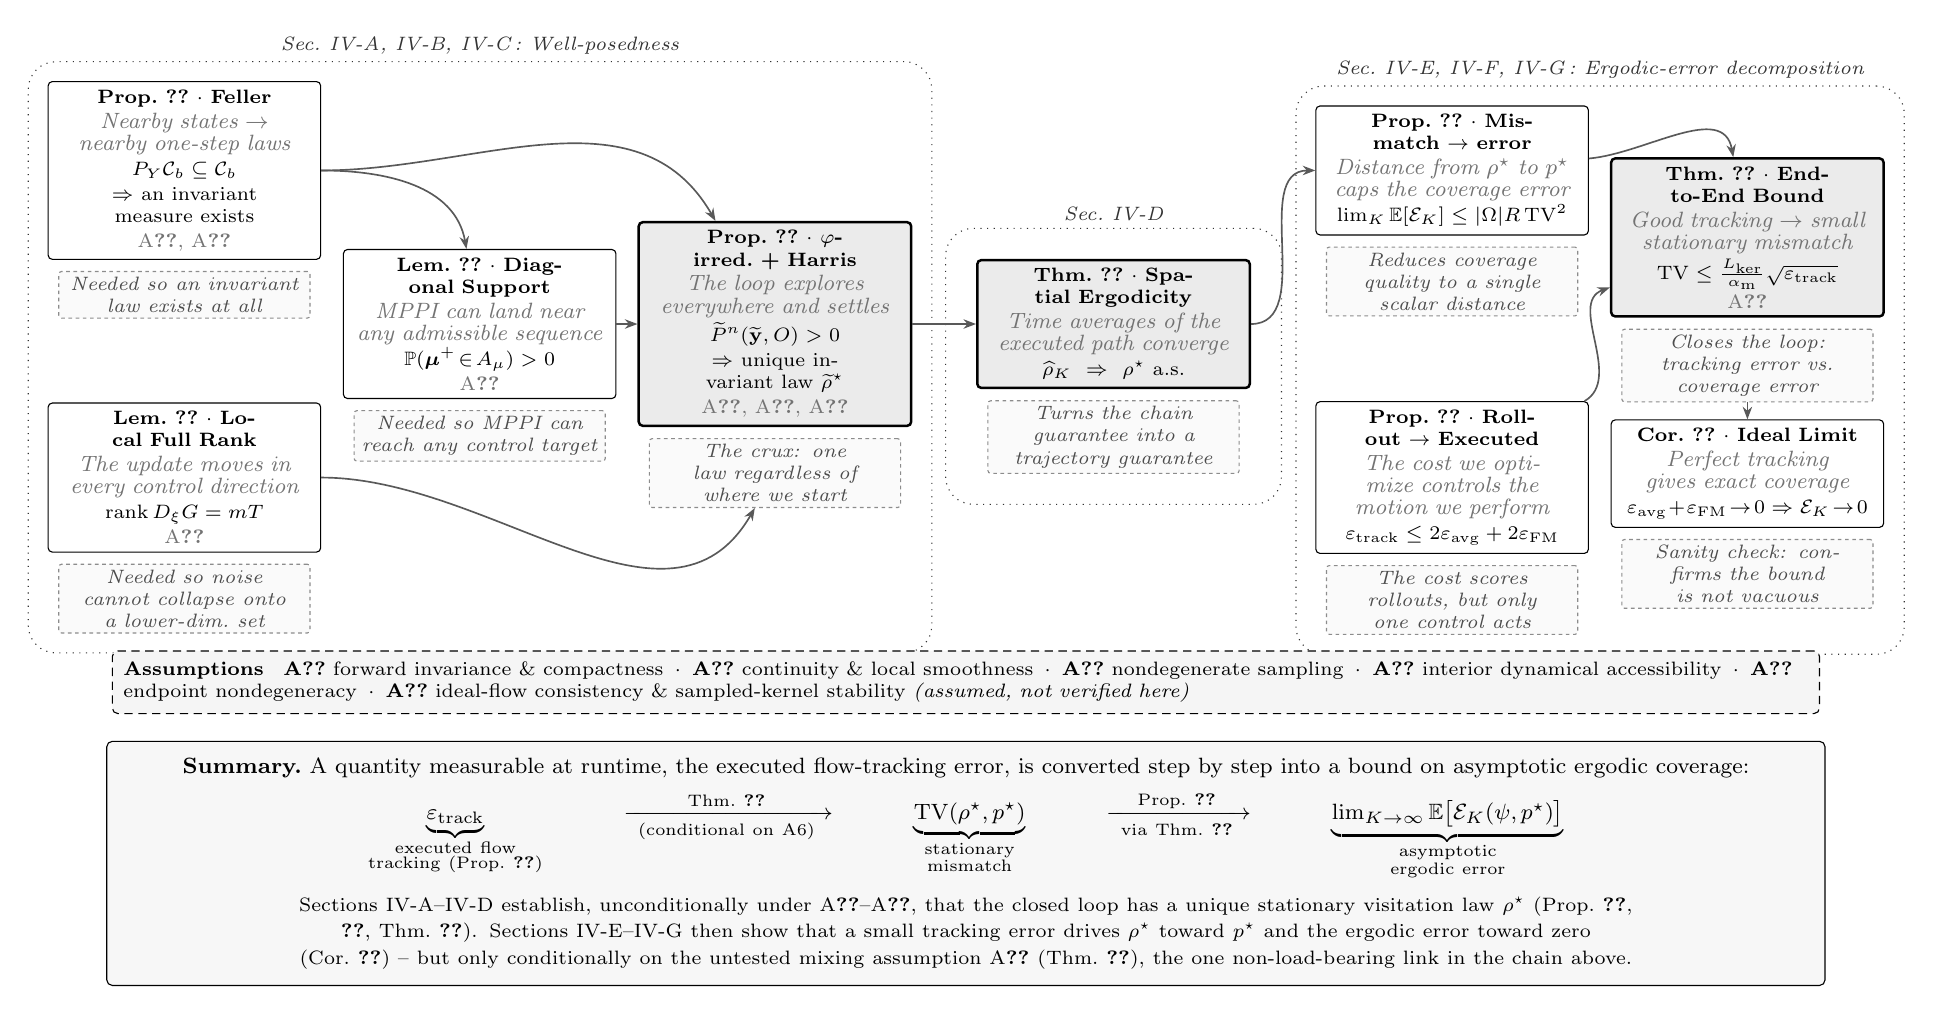
\begin{tikzpicture}[
  font=\scriptsize,
  >={Stealth[length=1.6mm]},
  res/.style={draw,rounded corners=1.5pt,fill=white,
              align=center,inner sep=3pt,text width=3.25cm},
  key/.style={draw,line width=0.9pt,rounded corners=1.5pt,fill=black!8,
              align=center,inner sep=3pt,text width=3.25cm},
  ar/.style={->,semithick,black!65},
  stage/.style={draw=black!80,dotted,rounded corners=10pt,inner sep=7pt},
  stageD/.style={draw=black!80,dotted,rounded corners=10pt,inner sep=11pt},
  why/.style={draw=black!45,dash pattern=on 1.3pt off 1.3pt,rounded corners=1pt,
              fill=black!2,align=center,inner sep=2pt,text width=3.05cm,
              font=\itshape\scriptsize,text=black!70},
]

%% ------------- results -------------
\node[res] (p1) at (0,1.95)
  {\textbf{Prop.~\ref*{prop:mppi_feller} $\cdot$ Feller}\\[1pt]
   \how{Nearby states $\to$ nearby one-step laws}\\[1pt]
   \mbox{$P_Y\mathcal C_b\subseteq\mathcal C_b$}\\[1pt]
   $\Rightarrow$ an invariant measure exists\\[1pt]\ustag{A\ref*{as:continuity}, A\ref*{as:sampling}}};
\node[res] (l2) at (0,-1.95)
  {\textbf{Lem.~\ref*{lem:diag_submersion} $\cdot$ Local Full Rank}\\[1pt]
   \how{The update moves in every control direction}\\[1pt]
   \mbox{$\operatorname{rank}D_\xi G=mT$}\\[1pt]\ustag{A\ref*{as:continuity}}};
\node[res] (l1) at (3.75,0)
  {\textbf{Lem.~\ref*{lem:diag_support} $\cdot$ Diagonal Support}\\[1pt]
   \how{MPPI can land near any admissible sequence}\\[1pt]
   \mbox{$\mathbb P(\boldsymbol\mu^+\!\in\!A_\mu)>0$}\\[1pt]\ustag{A\ref*{as:sampling}}};

\node[key] (p2) at (7.50,0)
  {\textbf{Prop.~\ref*{prop:mppi_irreducible} $\cdot$ $\varphi$-irred.\ + Harris}\\[1pt]
   \how{The loop explores everywhere and settles}\\[1pt]
   \mbox{$\widetilde P^n(\widetilde{\mathbf y},O)>0$}\\[1pt]
   $\Rightarrow$ unique invariant law $\widetilde\rho^\star$\\[1pt]\ustag{A\ref*{as:compactness}, A\ref*{as:accessibility}, A\ref*{as:endpoint}}};
\node[key] (t1) at (11.80,0)
  {\textbf{Thm.~\ref*{thm:closed_loop_ergodicity} $\cdot$ Spatial Ergodicity}\\[1pt]
   \how{Time averages of the executed path converge}\\[1pt]
   $\widehat\rho_K\Rightarrow\rho^\star$ a.s.};

\node[res] (p3) at (16.10,1.95)
  {\textbf{Prop.~\ref*{prop:ergodic_error_decomposition} $\cdot$ Mismatch $\to$ error}\\[1pt]
   \how{Distance from $\rho^\star$ to $p^\star$ caps the coverage error}\\[1pt]
   \mbox{$\lim_K\mathbb E[\mathcal E_K]\le|\Omega|R\,\mathrm{TV}^2$}};
\node[res] (p4) at (16.10,-1.95)
  {\textbf{Prop.~\ref*{prop:executed_flow_tracking} $\cdot$ Rollout $\to$ Executed}\\[1pt]
   \how{The cost we optimize controls the motion we perform}\\[1pt]
   \mbox{$\varepsilon_{\mathrm{track}}\le2\varepsilon_{\mathrm{avg}}+2\varepsilon_{\mathrm{FM}}$}};

\node[key] (t2) at (19.85,1.10)
  {\textbf{Thm.~\ref*{thm:end_to_end_ergodic_bound} $\cdot$ End-to-End Bound}\\[1pt]
   \how{Good tracking $\to$ small stationary mismatch}\\[1pt]
   \mbox{$\mathrm{TV}\le\tfrac{L_{\mathrm{ker}}}{\alpha_{\mathrm m}}\sqrt{\varepsilon_{\mathrm{track}}}$}\\[1pt]\ustag{A\ref*{as:ideal_kernel_stability}}};
\node[res] (c1) at (19.85,-1.90)
  {\textbf{Cor.~\ref*{cor:flow_matching_consistency} $\cdot$ Ideal Limit}\\[1pt]
   \how{Perfect tracking gives exact coverage}\\[1pt]
   \mbox{$\varepsilon_{\mathrm{avg}}\!+\!\varepsilon_{\mathrm{FM}}\!\to\!0\Rightarrow\mathcal E_K\!\to\!0$}};


%% ------------- why (rationale) callouts -------------
\node[why, below=0.14cm of p1] (p1w) {Needed so an invariant law exists at all};
\node[why, below=0.14cm of l2] (l2w) {Needed so noise cannot collapse onto a lower-dim.\ set};
\node[why, below=0.14cm of l1] (l1w) {Needed so MPPI can reach any control target};
\node[why, below=0.14cm of p2] (p2w) {The crux: one law regardless of where we start};
\node[why, below=0.14cm of t1] (t1w) {Turns the chain guarantee into a trajectory guarantee};
\node[why, below=0.14cm of p3] (p3w) {Reduces coverage quality to a single scalar distance};
\node[why, below=0.14cm of p4] (p4w) {The cost scores rollouts, but only one control acts};
\node[why, below=0.14cm of t2] (t2w) {Closes the loop: tracking error vs.\ coverage error};
\node[why, below=0.14cm of c1] (c1w) {Sanity check: confirms the bound is not vacuous};

\draw[ar] (p1) to[out=0,in=100]  (l1);
\draw[ar] (l1) -- (p2);
\draw[ar] (p1) to[out=0,in=120]   (p2);
\draw[ar] (l2) to[out=0,in=240]  (p2w);
\draw[ar] (p2) -- (t1);
\draw[ar] (t1) to[out=0,in=180]   (p3);
\draw[ar] (p3) to[out=5,in=100]   (t2);
\draw[ar] (p4) to[out=30,in=200]   (t2);
\draw[ar] (t2w) -- (c1);

%% ------------- stage backdrops -------------
\begin{scope}[on background layer]
  \node[stage,fit=(p1)(l2)(l1)(p2)(l2w),
        label={[font=\scriptsize\itshape,black!80,yshift=-1pt]above:Sec.~IV-A, IV-B, IV-C\,:\ Well-posedness}] {};
  \node[stageD,fit=(t1)(t1w),
        label={[font=\scriptsize\itshape,black!80,yshift=-1pt]above:Sec.~IV-D}] {};
  \node[stage,fit=(p3)(p4)(t2)(c1)(c1w)(p4w),
        label={[font=\scriptsize\itshape,black!80,yshift=-1pt]above:Sec.~IV-E, IV-F, IV-G\,:\ Ergodic-error decomposition}] {};
\end{scope}

%% ------------- assumption legend -------------
\node[draw,rounded corners=2pt,densely dashed,fill=black!4,inner sep=4pt,
      text width=21.4cm,align=left,font=\scriptsize] (leg) at (9.925,-4.55)
 {\textbf{Assumptions}\;\;
  \textbf{A\ref*{as:compactness}} forward invariance \& compactness\, $\cdot$\,
  \textbf{A\ref*{as:continuity}} continuity \& local smoothness\, $\cdot$\,
  \textbf{A\ref*{as:sampling}} nondegenerate sampling\, $\cdot$\,
  \textbf{A\ref*{as:accessibility}} interior dynamical accessibility\, $\cdot$\,
  \textbf{A\ref*{as:endpoint}} endpoint nondegeneracy\, $\cdot$\,
  \textbf{A\ref*{as:ideal_kernel_stability}} ideal-flow consistency \& sampled-kernel stability \emph{(assumed, not verified here)}};

%% ------------- goal banner -------------
\node[draw,rounded corners=2pt,fill=black!3,inner sep=6pt,text width=21.4cm,align=center,
      font=\footnotesize] (goal) at (9.925,-6.85)
  {\textbf{Summary.}\ A quantity measurable at runtime, the
   executed flow-tracking error, is converted step by step into a bound on
   asymptotic ergodic coverage:\\[4pt]
   $\underbrace{\varepsilon_{\mathrm{track}}}_{\substack{\text{executed flow}\\\text{tracking (Prop.~\ref*{prop:executed_flow_tracking})}}}
   \;\xrightarrow[\ \text{(conditional on A6)}\ ]{\ \text{Thm.~\ref*{thm:end_to_end_ergodic_bound}}\ }\;
   \underbrace{\mathrm{TV}(\rho^\star,p^\star)}_{\substack{\text{stationary}\\\text{mismatch}}}
   \;\xrightarrow[\ \text{via Thm.~\ref*{thm:closed_loop_ergodicity}}\ ]{\ \text{Prop.~\ref*{prop:ergodic_error_decomposition}}\ }\;
   \underbrace{\textstyle\lim_{K\to\infty}\mathbb E\big[\mathcal E_K(\psi,p^\star)\big]}_{\substack{\text{asymptotic}\\\text{ergodic error}}}$
   \\[5pt]
   \normalfont\scriptsize
   Sections~IV-A--IV-D establish, unconditionally under A\ref*{as:compactness}--A\ref*{as:endpoint}, that the closed
   loop has a unique stationary visitation law $\rho^\star$ (Prop.~\ref*{prop:mppi_feller}, \ref*{prop:mppi_irreducible}, Thm.~\ref*{thm:closed_loop_ergodicity}). Sections~IV-E--IV-G then show that a small tracking error drives
   $\rho^\star$ toward $p^\star$ and the ergodic error toward zero (Cor.~\ref*{cor:flow_matching_consistency}) --
   but only conditionally on the untested mixing assumption A\ref*{as:ideal_kernel_stability} (Thm.~\ref*{thm:end_to_end_ergodic_bound}), the
   one non-load-bearing link in the chain above.};

\end{tikzpicture}
\endgroup
}
\caption{\cl{Logical structure of Sec.~\ref{sec:guarantees}. Arrows denote
``is used in the proof of''; tags list the assumptions each result invokes.
Shaded boxes mark the three load-bearing results. Sections~\ref{sec:feller}--\ref{sec:irreducibility}
establish that the finite-sample \cl{memory-augmented} MPPI closed loop is positive Harris recurrent
(Prop.~\ref{prop:mppi_irreducible}), so that the executed trajectory admits a
unique asymptotic spatial visitation law $\rho^\star$
(Thm.~\ref{thm:closed_loop_ergodicity}). Sections~\ref{sec:asymptotic_error}--\ref{sec:stationary_coverage}
convert the residual mismatch between $\rho^\star$ and the target $p^\star$ into
asymptotic ergodic error along the chain shown at the bottom.
Proposition~\ref{prop:executed_flow_tracking} has no incoming edge: it is
self-contained, requiring only nonnegativity and normalization of the MPPI
weights. Theorem~\ref{thm:end_to_end_ergodic_bound} and
Corollary~\ref{cor:flow_matching_consistency} are conditional on
Assumption~\ref{as:ideal_kernel_stability}, which is stated but not established
in this work.}}
\label{fig:section_roadmap}
\end{figure*}

Since MPPI re-samples i.i.d.\ control perturbations at every replanning step and the next state depends on the past only through $(\mathbf{x}_t,\boldsymbol\mu_t\cl{,\mathcal M_t})$, the closed-loop process is a time-homogeneous Markov chain, with augmented state
\begin{equation}\label{eq:augmented_state}
    \mathbf Y_t := (\mathbf x_t,\boldsymbol\mu_t\cl{,\mathcal M_t})
    \in \mathcal Y := \mathcal X \times \mathcal U^T \cl{\times \mathcal Z^{P}} ,
\end{equation}
where $\mathcal X\subset\mathbb R^d$ is an admissible robot-state set\cl{,} $\mathcal U\subset\mathbb R^m$ the admissible control set\cl{, and $\mathcal Z:=\Omega_{\mathrm{free}}$ the projected workspace in which each of the $P$ fading-memory entries lives}. \cl{The memory component $\mathcal M_t$ evolves by the deterministic continuous shift~\eqref{eq:memory_shift}: it appends the newly executed projected state and drops the oldest, introducing no fresh randomness. It enters the transition kernel only through the continuous reference-flow cost of Sec.~\ref{sec:memory_flow}, and, being a bounded readout of the last $P$ physical states, preserves time-homogeneity.} \cl{Time homogeneity presumes that the target density, cost structure, and environment do not vary explicitly with $t$; time-varying quantities, such as moving obstacles or a drifting target, are accommodated only insofar as they are encoded in the state $\mathbf x_t$, so that the transition kernel itself remains fixed.} \cl{Throughout, we write $\mathcal{U}^\circ := \operatorname{int}(\mathcal{U})$ for the interior of the single-control set, so that $(\mathcal U^\circ)^T=\operatorname{int}(\mathcal U^T)$ is the set of nominal sequences lying strictly inside $\mathcal{U}^T$; we call these the \emph{admissible nominal targets}. On $(\mathcal U^\circ)^T$ saturation
leaves a target unchanged, so aiming at such a point and executing it coincide; only on the boundary $\partial(\mathcal{U}^T)$ would saturation clip the target.} \mm{With this notation, the augmented rollout cost $\bar S^{(b)}(\mathbf x_t,\boldsymbol\mu_t,\Xi_t)$ of~\eqref{eq:S_augmented} is written compactly as $\bar S^{(b)}(\mathbf Y,\Xi_t)$, and similarly for its constituent task cost $S^{(b)}$ and for the weights below.}
Let $P_Y$ denote the Markov transition kernel of one finite-sample MPPI replanning step on $\mathcal Y$, comprising rollout sampling, cost evaluation, importance weighting, the nominal-sequence update, execution of the first control $\boldsymbol\mu^+_{t,0}$, horizon shifting\cl{, and the fading-memory shift~\eqref{eq:memory_shift}}.

\cl{At each replanning step, fresh perturbations $\Xi_t$ update the warm start
$\boldsymbol\mu_t$ into $\boldsymbol\mu_t^+$. Its first control is executed, and
the remaining controls are shifted and padded to form
$\boldsymbol\mu_{t+1}$, which serves as the warm start for the next MPPI update\cl{; the executed state simultaneously enters the fading memory}.}

\cl{To characterize the nominal sequence at a generic pre-update instant
$t\geq1$, we write it directly as the result of the preceding shift. For a
continuous deterministic padding rule
$\widehat{\zeta}:\mathcal U^{T-1}\to\mathcal U$ that depends only on the
retained tail,}
\begin{equation}\label{eq:shift_map}
    \cl{\boldsymbol\mu_t
    =
    \Big(
    \boldsymbol\mu^+_{t-1,1},\ldots,\boldsymbol\mu^+_{t-1,T-1},
    \widehat{\zeta}\big(
    \boldsymbol\mu^+_{t-1,1},\ldots,\boldsymbol\mu^+_{t-1,T-1}
    \big)
    \Big).}
\end{equation}
\cl{This includes, for example, repeat-last and fixed-value padding. Define the
retained part of the current warm start as}
\begin{equation}\label{eq:reduced_nominal}
    \cl{\widetilde{\boldsymbol\mu}_t
    :=
    \big(
    \boldsymbol\mu_{t,0},\ldots,\boldsymbol\mu_{t,T-2}
    \big)
    =
    \big(
    \boldsymbol\mu^+_{t-1,1},\ldots,
    \boldsymbol\mu^+_{t-1,T-1}
    \big).}
\end{equation}
\cl{The complete warm start is therefore reconstructed as}
\begin{equation}\label{eq:nominal_reconstruction}
    \cl{\boldsymbol\mu_t
    =
    \Big(
    \widetilde{\boldsymbol\mu}_t,
    \widehat{\zeta}(\widetilde{\boldsymbol\mu}_t)
    \Big).}
\end{equation}
\cl{Thus, at every pre-update instant after initialization, the final control
slot is determined by the retained part and cannot vary independently. This
does not restrict the subsequent MPPI update, which uses fresh perturbations to
update the complete sequence.}

\cl{The possible pre-update sequences are therefore confined to a
lower-dimensional subset of $\mathcal U^T$. Indeed, once
$\widetilde{\boldsymbol\mu}_t\in\mathcal U^{T-1}$ is specified, the final slot
can only take the single value
$\widehat{\zeta}(\widetilde{\boldsymbol\mu}_t)$, rather than varying
independently over $\mathcal U$. A single value has zero $m$-dimensional
Lebesgue measure, and integrating over all possible retained sequences therefore
gives zero $mT$-dimensional Lebesgue measure. Consequently, the chain cannot be
irreducible with respect to Lebesgue measure on
$\mathcal Y=\mathcal X\times\mathcal U^T\cl{\times\mathcal Z^P}$. We instead analyze the reduced
state}
\begin{equation}\label{eq:reduced_state}
    \cl{\widetilde{\mathbf Y}_t
    :=
    \big(
    \mathbf x_t,\widetilde{\boldsymbol\mu}_t\cl{,\mathcal M_t}
    \big)
    \in
    \widetilde{\mathcal Y}
    :=
    \mathcal X\times\mathcal U^{T-1}\cl{\times\mathcal Z^{P}}.}
\end{equation}
\cl{The reconstruction in \eqref{eq:nominal_reconstruction} gives a continuous
one-to-one correspondence between $\widetilde{\mathcal Y}$ and the invariant
pre-update state space of the original chain. Hence,
$\{\widetilde{\mathbf Y}_t\}$ is again a time-homogeneous Markov chain, and its
results transfer to the original chain through this reconstruction.} \cl{The
fading memory $\mathcal M_t$ is retained in the reduced state because the
transition depends on it; unlike the nominal tail it is not collapsed, but it is
a deterministic continuous function of the last $P$ executed positions (a delay
embedding), so it adds no independent stochastic direction. We revisit this
point in the proof of Prop.~\ref{prop:mppi_irreducible}.}

\cl{The well-posedness analysis relies on the following conditions on the
finite-sample \cl{memory-augmented} MPPI closed loop, which we state as separate assumptions and
refer to individually. The first three concern the regularity of the
controller, and the last two the reachability of the robot dynamics.}

\begin{assumption}[Forward invariance and compactness]
\label{as:compactness}
There exist compact admissible sets
$\mathcal X\subset\mathbb R^d$ and
$\mathcal U\subset\mathbb R^m$, both with nonempty interior, such that the
one-step closed-loop transition, including control saturation\cl{,}
nominal-sequence shifting\cl{, and the fading-memory shift~\eqref{eq:memory_shift}}, maps
$\mathcal Y:=\mathcal X\times\mathcal U^T\cl{\times\mathcal Z^P}$
into itself for every perturbation realization. The projected free workspace
$\mathcal Z=\Omega_{\mathrm{free}}:=\Pi(\mathcal X)\subseteq\Omega$ is compact and connected\cl{, so the fading-memory space $\mathcal Z^P$ is compact}.
\end{assumption}

\begin{assumption}[Continuity and local smoothness]
\label{as:continuity}
The discretized dynamics $f_d$, spatial projection $\Pi$, control saturation,
nominal-sequence shift, \cl{the fading-memory shift~\eqref{eq:memory_shift}, the fading occupancy density~\eqref{eq:occupancy_density} and the induced reference flow $\widetilde{\mathbf h}^{\mathcal M}_t$,} and rollout costs are continuous. All rollout costs are
finite for every admissible state, nominal sequence, \cl{fading memory,} and perturbation
realization, and saturation acts as the identity on $\mathcal U^\circ$.
Moreover, the reduced one-step transition map, comprising the dynamics, the
nominal-update map $G(\mathbf Y,\Xi):=\boldsymbol\mu^+$, saturation, \cl{the memory shift,} and the
shift/padding map, is jointly continuously differentiable in
$(\widetilde{\mathbf Y},\Xi)$ in a neighborhood of every finite diagonal-witness
trajectory used in Sec.~\ref{sec:irreducibility}.
\end{assumption}

\cl{For the reference field of Sec.~\ref{sec:memory_flow}, global continuity
follows from the continuity of the kernel, dynamics, projection,
positive-part function, and finite sums defining the occupancy and memory
fields. The denominators in~\eqref{eq:relative_excess} and
\eqref{eq:excess_masses} are bounded below by $\varepsilon_p$ and
$\varepsilon_S$, respectively, while the regularized speed
gauge~\eqref{eq:speed_gauge} is continuous. Compactness then implies
boundedness of the resulting reference field. These properties provide the
continuity required by the Feller argument of Sec.~\ref{sec:feller}.}

\cl{The transition map is only piecewise continuously differentiable. Its
nonsmooth sets include the occupancy-coincidence surfaces
$o_t^{h_q}(\mathbf m_{t,i})=p_{h_q}^\star(\mathbf m_{t,i})$ and the
regularization boundary at which the norm of the input to $\Pi_v$ equals
$\varepsilon_v$. Accordingly, the local differentiability clause of
Assumption~\ref{as:continuity} requires the finite diagonal-witness
neighbourhoods used in Sec.~\ref{sec:irreducibility} not to intersect these
sets. This is a local regularity requirement, not a consequence of global
continuity. If global $C^1$ regularity is desired, the positive part may be
replaced by its squared positive part and the max-based speed gauge by a smooth
normalization.}

\begin{assumption}[Nondegenerate sampling]
\label{as:sampling}
The rollout count satisfies $1\leq N<\infty$, the temperature satisfies
$\lambda>0$, and the complete rollout perturbation sequences are sampled
independently from a Gaussian distribution with positive-definite covariance.
\end{assumption}

\begin{assumption}[Interior dynamical accessibility]
\label{as:accessibility}
For every $\mathbf x\in\mathcal X$ and every nonempty relatively open set
$O_{\mathbf x}\subseteq\mathcal X$, there exist $n\in\mathbb N$ and a control
sequence
$(\mathbf u_0,\ldots,\mathbf u_{n-1})\in\operatorname{int}(\mathcal U)^n$
whose deterministic trajectory remains in $\mathcal X$ and satisfies
$\mathbf x_n\in O_{\mathbf x}$.
\end{assumption}

\begin{assumption}[Endpoint nondegeneracy]
\label{as:endpoint}
There exists $n^\ast\in\mathbb N$ such that, for every
$\mathbf x\in\mathcal X$, the endpoint map
\begin{equation}\label{eq:endpoint_map}
    E_{\mathbf x}:
    (\mathbf u_0,\ldots,\mathbf u_{n^\ast-1})
    \longmapsto
    f_d^{(n^\ast)}
    \big(
    \mathbf x,\mathbf u_0,\ldots,\mathbf u_{n^\ast-1}
    \big)
\end{equation}
is continuously differentiable and has Jacobian of full row rank $d$ at some
admissible sequence
$\mathbf u^\star(\mathbf x)\in\operatorname{int}(\mathcal U^{n^\ast})$.
\end{assumption}

\cl{Assumption~\ref{as:compactness} confines the analysis to a bounded
forward-invariant operating region\cl{, now including the compact fading-memory space $\mathcal Z^P$}. The global continuity in
Assumption~\ref{as:continuity} ensures that the closed-loop transition
varies continuously with its current state\cl{, fading memory,} and perturbations, while the local
joint-smoothness clause is used to establish full rank of the multistep
perturbation-to-state map near the diagonal witnesses. Assumption~\ref{as:sampling} gives the
perturbation law full support, assigning positive probability to every
nonempty open subset of the perturbation space.}

\cl{The final two conditions concern the robot dynamics.
Assumption~\ref{as:accessibility} ensures that interior admissible controls can steer
the deterministic state toward any region of the chosen operating set. It does
not claim that MPPI will select those controls; this is established separately
by Lemma~\ref{lem:diag_support}. Assumption~\ref{as:endpoint} ensures
that, over a finite number of steps, small control variations generate
variations in every physical-state direction. This prevents the state law from
remaining confined to a lower-dimensional subset of $\mathcal X$\cl{; because the fading memory is a delay embedding of past executed positions, the same mechanism steers the memory window to any target configuration, as detailed in Prop.~\ref{prop:mppi_irreducible}}.}

\cl{These conditions enter the analysis progressively.
Sec.~\ref{sec:feller} uses compactness and continuity to establish the Feller
property and hence existence of an invariant probability measure.
Sec.~\ref{sec:global_support} combines continuity with nondegenerate sampling
to prove global support of the MPPI nominal update. Finally,
Sec.~\ref{sec:irreducibility} combines this support with local smoothness,
dynamical accessibility, and endpoint nondegeneracy to establish
$\varphi$-irreducibility and positive Harris recurrence.}

\subsection{Feller Property}
\label{sec:feller}
We begin with the Feller property, since it is the structural prerequisite for the irreducibility result that follows. \cl{Concretely, it asks that nearby augmented states produce nearby one-step distributions, so that small perturbations to the robot state\cl{, fading memory,} or nominal sequence cannot cause abrupt changes in the controller's stochastic response.}

\begin{proposition}[Feller property of finite-sample MPPI]
\label{prop:mppi_feller}
Under Assumptions~\ref{as:compactness}--\ref{as:endpoint}, the closed-loop transition
kernel $P_Y$ is Feller on $\mathcal{Y}$, namely for every bounded continuous
$g:\mathcal{Y}\to\mathbb{R}$,
\begin{equation}
    P_Y g(\mathbf{Y})
    :=
    \mathbb{E}\!\left[g(\mathbf{Y}_{t+1})\mid\mathbf{Y}_t=\mathbf{Y}\right]
\end{equation}
is continuous in $\mathbf{Y}$.
\end{proposition}

\begin{proof}
Let $g\in\mathcal{C}_b(\mathcal{Y})$, and \mm{recall $\Xi_t$ (the i.i.d.\ rollout perturbations) from~\eqref{eq:Xi_def}}. The one-step MPPI update defines the random map $\mathbf{Y}_{t+1}=F(\mathbf{Y}_t,\Xi_t)$, where $F$ denotes the complete closed-loop transition (as opposed to the nominal-update map $G$ of Assumption~\ref{as:continuity}), so that
\begin{equation}
    P_Y g(\mathbf{Y}) = \mathbb{E}\!\left[g(F(\mathbf{Y},\Xi_t))\right].
\end{equation}
\cl{We must show that $P_Y g$ is continuous for every $g\in\mathcal{C}_b(\mathcal{Y})$. We first prove that the frozen-noise map $F(\,\cdot\,,\xi)$ is continuous for every fixed $\xi$, and then pass this pathwise continuity through the expectation by dominated convergence.}

By Assumption~\ref{as:continuity}, every intermediate quantity entering the MPPI update (sampled controls, rollout states, \cl{the fading occupancy density and reference flow $\widetilde{\mathbf h}^{\mathcal M}_t$,} shaped costs $\bar{S}^{(b)}(\mathbf{Y},\xi)$, importance weights, weighted control update, executed control, shifted nominal sequence\cl{, and the shifted fading memory~\eqref{eq:memory_shift}}) depends continuously on $\mathbf{Y}$. For the weights, continuity follows from $N<\infty$ and $\lambda>0$ (Assumption~\ref{as:sampling}), which ensure a strictly positive denominator in
\begin{equation}
    w^{(b)}(\mathbf{Y},\xi)
    =
    \frac{
        \exp\!\left(-\bar{S}^{(b)}(\mathbf{Y},\xi)/\lambda\right)
    }{
        \sum_{j=1}^{N}\exp\!\left(-\bar{S}^{(j)}(\mathbf{Y},\xi)/\lambda\right)
    }.
\end{equation}
By composition of continuous maps, $F(\,\cdot\,,\xi)$ is therefore continuous for every fixed $\xi$\cl{; in particular the deterministic memory shift, being continuous, composes into $F(\,\cdot\,,\xi)$ without affecting the argument}.

\cl{Now let $\mathbf{Y}_n\to\mathbf{Y}$. Since $F(\,\cdot\,,\xi)$ is continuous for every realization $\xi$ of $\Xi_t$, we have $F(\mathbf{Y}_n,\Xi_t)\to F(\mathbf{Y},\Xi_t)$ almost surely (a.s.), and continuity of $g$ gives}
\begin{equation}
    g(F(\mathbf{Y}_n,\Xi_t))\longrightarrow g(F(\mathbf{Y},\Xi_t))
    \qquad\text{a.s.}
\end{equation}
Since $g\in\mathcal{C}_b(\mathcal{Y})$, there exists $M<\infty$ such that $|g(y)|\le M$ for all $y\in\mathcal{Y}$, providing an integrable dominating constant. Dominated convergence therefore yields
\begin{equation}
\begin{aligned}
    \lim_{n\to\infty} P_Y g(\mathbf{Y}_n)
    &=
    \lim_{n\to\infty}\mathbb{E}\!\left[g(F(\mathbf{Y}_n,\Xi_t))\right]\\
    &=
    \mathbb{E}\!\left[\lim_{n\to\infty}g(F(\mathbf{Y}_n,\Xi_t))\right]\\
    &=
    \mathbb{E}\!\left[g(F(\mathbf{Y},\Xi_t))\right]\\
    &=
    P_Y g(\mathbf{Y}),
\end{aligned}
\end{equation}
so $P_Y g\in\mathcal{C}_b(\mathcal{Y})$ for every $g\in\mathcal{C}_b(\mathcal{Y})$, and $P_Y$ is Feller.
\end{proof}

\subsection{\texorpdfstring{\cl{Global Support of the MPPI Update}}{Global Support of the MPPI Update}}
\label{sec:global_support}

\cl{Our next objective is to establish $\varphi$-irreducibility of the reduced
augmented chain
$\widetilde{\mathbf Y}_t=(\mathbf x_t,\widetilde{\boldsymbol\mu}_t\cl{,\mathcal M_t})$. The first
step is to show that the chain can reach any open region of this joint
state-control\cl{-memory} space. Dynamical accessibility will provide control sequences
that steer $\mathbf x_t$ toward a desired physical region\cl{, and hence the fading-memory window through the corresponding positions}, but MPPI does not
execute a prescribed sequence directly. We must therefore show that, from any
current augmented state, the finite-sample MPPI update assigns positive
probability to every open neighborhood of an admissible control sequence. Its
first slot can then approximate the required executed control, while its
remaining slots determine the next warm start.}

\cl{This control-space support is not automatic: MPPI draws $N$ Gaussian
perturbation sequences, reweights them by their rollout costs, and averages
them, so the weighted update could in principle fail to cover parts of the
admissible control space. The following lemma rules out this obstruction using
a diagonal configuration in which all rollouts receive the same complete
perturbation sequence. The rollouts then have identical controls, trajectories,
and costs, giving uniform weights and an update that reproduces the common
perturbation exactly. Although the exact diagonal configuration has
probability zero, continuity maps a neighborhood of it into a neighborhood of the desired
nominal sequence, and this perturbation neighborhood has positive probability
under the full-rank Gaussian sampling law.}

\begin{lemma}[\cl{Diagonal global support of the MPPI nominal update}]
\label{lem:diag_support}
\cl{Under Assumptions~\ref{as:compactness}--\ref{as:endpoint}, for every
$\mathbf Y=(\mathbf x_t,\boldsymbol\mu_t\cl{,\mathcal M_t})\in\mathcal Y$ and every nonempty open
set
$A_{\mu}\subseteq\operatorname{int}(\mathcal U^T)$,}
\begin{equation}
    \cl{\mathbb P\!\left(
        \boldsymbol\mu_t^+\in A_{\mu}
        \mid \mathbf Y_t=\mathbf Y
    \right)>0.}
\end{equation}
\end{lemma}

\begin{proof}
\cl{We first identify one perturbation configuration that produces an arbitrary
target sequence in $A_{\mu}$ exactly. Since this individual configuration has
probability zero, we then use continuity to expand it into a
positive-probability neighborhood. The fading memory $\mathcal M_t$ enters the rollout costs but not the mechanism below, which produces the target nominal sequence for any fixed $\mathcal M_t$.}

\cl{\textit{Step 1: construct an exact diagonal witness.}
Choose any target sequence $\bar{\boldsymbol\mu}\in A_{\mu}$ and define the
complete perturbation required to move the current nominal sequence to this
target,}
\begin{equation}
    \cl{\bar{\boldsymbol\epsilon}
    :=
    \bar{\boldsymbol\mu}-\boldsymbol\mu_t.}
\end{equation}
\cl{We consider the joint perturbation configuration in which every rollout
receives this same complete sequence,}
\begin{equation}\label{eq:diag_witness}
    \cl{\bar{\boldsymbol\epsilon}^{(b)}
    =
    \bar{\boldsymbol\epsilon},
    \qquad b=1,\ldots,N,}
\end{equation}
\cl{and denote it by
$\bar\Xi=(\bar{\boldsymbol\epsilon},\ldots,
\bar{\boldsymbol\epsilon})\in\mathbb R^{NTm}$. Equality here is across
rollouts: the perturbation may still vary along the prediction horizon.}

\cl{Since $\bar{\boldsymbol\mu}$ lies in the interior of $\mathcal U^T$,
saturation is inactive, and every rollout uses the target control sequence}
\begin{equation}
    \cl{\mathbf u^{(b)}
    =
    \boldsymbol\mu_t+\bar{\boldsymbol\epsilon}^{(b)}
    =
    \bar{\boldsymbol\mu}.}
\end{equation}
\cl{All rollouts start from the same state and use the same deterministic
rollout model. They therefore generate identical trajectories and identical
values of every term entering the importance weights\cl{, including the shared fading-memory-based flow cost}. Consequently,}
\begin{equation}
    \cl{w^{(b)}(\mathbf Y,\bar\Xi)=\frac{1}{N},
    \qquad b=1,\ldots,N.}
\end{equation}
\cl{Substituting the common perturbation and uniform weights into the MPPI
update gives}
\begin{equation}\label{eq:diag_exact}
    \cl{\boldsymbol\mu_t^+}
    =
    \cl{\boldsymbol\mu_t
    +
    \sum_{b=1}^{N}
    \frac{1}{N}
    \big(
    \bar{\boldsymbol\mu}-\boldsymbol\mu_t
    \big)} =
    \cl{\bar{\boldsymbol\mu}.}
\end{equation}
\cl{Thus, for every target
$\bar{\boldsymbol\mu}\in A_{\mu}$, there exists a perturbation configuration
$\bar\Xi$ that produces it exactly, independently of the state\cl{, memory,} and cost
landscape. This does not mean that the sampler generates $\bar\Xi$ with
positive probability: as a single point under a continuous Gaussian law,
$\bar\Xi$ has probability zero.}




\cl{\textit{Step 2: expand the witness into a positive-probability
neighborhood.}
Step~1 identifies a single perturbation configuration $\bar\Xi$ that produces
the target $\bar{\boldsymbol\mu}$ exactly. However, a single point has
probability zero under the continuous Gaussian sampling law, so this exact
witness alone does not establish the desired positive-probability result. We
therefore use continuity to show that all perturbation configurations
sufficiently close to $\bar\Xi$ also produce outputs in $A_{\mu}$.}

\cl{Let $G(\mathbf Y,\xi):=\boldsymbol\mu_t^+$ denote the nominal update as a
function of the joint perturbation vector. Since $A_{\mu}$ is open and contains
$\bar{\boldsymbol\mu}$, there exists $r>0$ such that}
\begin{equation}
    \cl{B_r(\bar{\boldsymbol\mu})\subseteq A_{\mu}.}
\end{equation}
\cl{By Assumptions~\ref{as:compactness}--\ref{as:endpoint},
$G(\mathbf Y,\cdot)$ is continuous, as established in the proof of
Proposition~\ref{prop:mppi_feller}. Since
$G(\mathbf Y,\bar\Xi)=\bar{\boldsymbol\mu}$, there exists $\delta>0$ such that}
\begin{equation}\label{eq:diag_neighborhood}
    \cl{\Xi\in B_\delta(\bar\Xi)
    \quad\Longrightarrow\quad
    G(\mathbf Y,\Xi)\in B_r(\bar{\boldsymbol\mu})
    \subseteq A_{\mu}.}
\end{equation}
\cl{Thus, the rollouts need not receive exactly the same perturbation. It is
enough for their joint perturbation configuration to lie sufficiently close to
the diagonal witness.}

\cl{The joint perturbation $\Xi_t$ has a full-rank Gaussian covariance and
therefore a strictly positive density on $\mathbb R^{NTm}$. The open ball
$B_\delta(\bar\Xi)$ consequently has strictly positive probability. Using
\eqref{eq:diag_neighborhood} and the independence of $\Xi_t$ from the current
state gives}
\begin{equation}
    \mathbb P\!\left(
        \boldsymbol\mu_t^+\in A_{\mu}
        \mid \mathbf Y_t=\mathbf Y
    \right)
    \geq
    \mathbb P\!\left(
        \Xi_t\in B_\delta(\bar\Xi)
    \right)
    >
    0.
\end{equation}
\end{proof}

\cl{Lemma~\ref{lem:diag_support} shows that every open region of the admissible
nominal-sequence space has positive probability, but it does not characterize
how many independent output directions are generated locally by the map
$G(\mathbf Y,\cdot)$. Its Jacobian maps $NmT$ perturbation directions into
$mT$ nominal-sequence directions, and therefore has rank at most $mT$. For the
Lebesgue-irreducibility argument, we must show that this maximum rank is
actually attained. Otherwise, the local outputs could vary in fewer than
$mT$ directions. For example, the map
$(z_1,z_2)\mapsto(z_1,0)$ has rank one and confines a two-dimensional Gaussian
input to a line in the output space.}

\begin{lemma}[\cl{Local nondegeneracy of the MPPI nominal update}]
\label{lem:diag_submersion}
\cl{Under Assumption~\ref{as:continuity}, the nominal-update map satisfies}
\begin{equation}
    \cl{\operatorname{rank}
    D_\xi G(\mathbf Y,\bar\Xi)=mT}
\end{equation}
\cl{at every diagonal witness $\bar\Xi$.}
\end{lemma}

\begin{proof}
\cl{For any $\mathbf h\in\mathbb R^{mT}$, define the common rollout variation}
\begin{equation}
    \cl{\mathbf H_{\mathrm{diag}}(\mathbf h)
    :=
    (\mathbf h,\ldots,\mathbf h)
    \in\mathbb R^{NmT}.}
\end{equation}
\cl{For $\mathbf h$ sufficiently small, the perturbed configuration
$\bar\Xi+\mathbf H_{\mathrm{diag}}(\mathbf h)$ remains diagonal and saturation
remains inactive. All rollouts are therefore still identical, their weights
remain equal to $1/N$, and the MPPI update satisfies exactly}
\begin{equation}
    \cl{G\big(
        \mathbf Y,
        \bar\Xi+\mathbf H_{\mathrm{diag}}(\mathbf h)
    \big)
    =
    G(\mathbf Y,\bar\Xi)+\mathbf h.}
\end{equation}
\cl{Differentiating with respect to $\mathbf h$ at
$\mathbf h=\mathbf0$ gives}
\begin{equation}
    \cl{D_\xi G(\mathbf Y,\bar\Xi)\,
    \mathbf H_{\mathrm{diag}}(\mathbf h)
    =
    \mathbf h.}
\end{equation}
\cl{Here,
$\mathbf H_{\mathrm{diag}}(\mathbf h):=(\mathbf h,\ldots,\mathbf h)$ applies
the same variation to all $N$ rollouts. Since every output direction
$\mathbf h$ can be generated in this way, the derivative is surjective and has
rank $mT$. Hence, $G(\mathbf Y,\cdot)$ is a submersion at $\bar\Xi$, meaning
that it locally spans every direction of the nominal-sequence space, although
different perturbation directions may produce the same output.}
\end{proof}

\cl{The map may discard perturbation directions that only change the
differences among rollouts, but it retains all directions needed to vary the
updated nominal sequence. This controller-side full-rank property can
therefore be combined with endpoint nondegeneracy to obtain a
full-dimensional perturbation-to-state map.}

\cl{Lemma~\ref{lem:diag_support} and
Lemma~\ref{lem:diag_submersion} establish two complementary controller-side
properties: MPPI can reach every open neighborhood of an interior admissible
control sequence, and its update retains all local control-sequence directions
near the corresponding diagonal witness. These results do not yet concern the
physical state. Dynamical accessibility and endpoint nondegeneracy connect the
sampled controls to the state evolution\cl{, and hence to the fading-memory window,} and complete the
$\varphi$-irreducibility argument.}

%============================================================
% INTUITIVE INTRODUCTION TO PROPOSITION 2
% ============================================================
\subsection{\texorpdfstring{\cl{$\varphi$-Irreducibility and Positive Harris Recurrence}}{phi-Irreducibility and Positive Harris Recurrence}}
\label{sec:irreducibility}

\cl{The Feller argument already guarantees existence of an invariant
probability measure. We now show that the reduced closed-loop chain cannot
remain confined to different invariant regions depending on its initialization.
This gives a unique invariant law and well-defined long-run visitation
statistics.}

\cl{The argument combines a global and a local property. Globally,
Assumption~\ref{as:accessibility} provides control sequences that reach any
physical-state region, while Lemma~\ref{lem:diag_support} ensures that MPPI can
approximate them with positive probability. Locally,
Lemma~\ref{lem:diag_submersion} and
Assumption~\ref{as:endpoint} transfer the Gaussian perturbations through
the MPPI update and the robot dynamics without losing any state-space
direction. This gives the transition kernel a full-dimensional continuous
component, which upgrades accessibility of open sets to
$\varphi$-irreducibility.} \cl{The fading memory is handled separately, at the end of the proof, as a deterministic delay readout of the executed positions.}

\begin{proposition}[\cl{$\varphi$-irreducibility and positive Harris recurrence}]
\label{prop:mppi_irreducible}
\cl{Under Assumptions~\ref{as:compactness}--\ref{as:endpoint}, the reduced closed-loop chain
$\{\widetilde{\mathbf Y}_t\}$ \cl{on $\widetilde{\mathcal Y}=\mathcal X\times\mathcal U^{T-1}\times\mathcal Z^P$} is $\varphi$-irreducible, with maximal
irreducibility measure of full topological support on \cl{the reachable subset of} $\widetilde{\mathcal Y}$,
and is positive
Harris recurrent. It therefore admits a unique invariant probability measure
$\widetilde\rho^\star$.}
\end{proposition}

\begin{proof}
\cl{The argument has three steps: accessibility of open sets\cl{ (including the memory window)}, local
full-dimensionality of the transition law, and positive Harris recurrence.}

\cl{\textit{Step 1: accessibility of open sets.}
Fix
$\widetilde{\mathbf Y}_0=(\mathbf x_0,\widetilde{\boldsymbol\mu}_0\cl{,\mathcal M_0})$ and a
nonempty open set $O\subseteq\widetilde{\mathcal Y}$. Choose a nonempty open
rectangle
$O_{\mathbf x}\times O_{\boldsymbol\mu}\cl{\times O_{\mathcal M}}\subseteq O$, with
$O_{\boldsymbol\mu}\subseteq\operatorname{int}(\mathcal U^{T-1})$\cl{ and $O_{\mathcal M}\subseteq\mathcal Z^P$ a product of position windows}. By
Assumption~\ref{as:accessibility}, there is an interior admissible sequence
$\mathbf u^\star=(\mathbf u^\star_0,\ldots,\mathbf u^\star_{n-1})$ steering
$\mathbf x_0$ into $O_{\mathbf x}$. Continuity of the $n$-step dynamics gives
$\eta>0$ such that any sequence satisfying
$\|\mathbf u_j-\mathbf u^\star_j\|<\eta$ also ends in $O_{\mathbf x}$; choose
$\eta$ small enough that
$B_\eta(\mathbf u^\star_j)\subseteq\operatorname{int}(\mathcal U)$.}

\cl{\textit{Reaching the memory window.} Because $\mathcal M_t$ records the last
$P$ executed positions, a target memory window in $O_{\mathcal M}$ is realized by
steering the executed trajectory through the corresponding $P$ positions. By
Assumption~\ref{as:accessibility} applied successively, and by the same
continuity estimate, there is an interior control sequence of length $P$ whose
executed positions land inside the prescribed windows; concatenating it after the
sequence reaching $O_{\mathbf x}$ shows that, over $n+P$ steps, the executed
trajectory can be steered so that both $\mathbf x_{n+P}\in O_{\mathbf x}$ and
$\mathcal M_{n+P}\in O_{\mathcal M}$. For notational brevity we absorb these $P$
extra steps into $n$ below.}

\cl{Only the first slot of each updated sequence is executed. We therefore
require this slot to follow $\mathbf u^\star_j$, while leaving the unused tail
free until the final step. Fix any nonempty open
$V\subseteq\operatorname{int}(\mathcal U^{T-1})$ and define}
\begin{equation}\label{eq:accessibility_nominal_sets}
\begin{aligned}
    \cl{A_j}
    &\cl{:=
    B_\eta(\mathbf u^\star_j)\times V,
    \qquad j=0,\ldots,n-2,}\\
    \cl{A_{n-1}}
    &\cl{:=
    B_\eta(\mathbf u^\star_{n-1})
    \times O_{\boldsymbol\mu}.}
\end{aligned}
\end{equation}
\cl{If $\boldsymbol\mu_j^+\in A_j$ for every $j$, the executed controls remain
within $\eta$ of $\mathbf u^\star$, so
$\mathbf x_n\in O_{\mathbf x}$\cl{ and $\mathcal M_n\in O_{\mathcal M}$}. At the final step, the tail of
$\boldsymbol\mu_{n-1}^+$ becomes
$\widetilde{\boldsymbol\mu}_n$, giving
$\widetilde{\boldsymbol\mu}_n\in O_{\boldsymbol\mu}$. Hence
$\widetilde{\mathbf Y}_n\in O$. Each $A_j$ is a nonempty open subset of
$\operatorname{int}(\mathcal U^T)$, so
Lemma~\ref{lem:diag_support} assigns every event
$\{\boldsymbol\mu_j^+\in A_j\}$ positive conditional probability from every
current state. Applying the tower property over the finite sequence yields}
\begin{equation}\label{eq:open_set_accessibility}
    \cl{\widetilde P^{\,n}
    (\widetilde{\mathbf Y}_0,O)>0.}
\end{equation}

\cl{\textit{Step 2: a full-dimensional continuous component.}
Accessibility of open sets does not yet exclude transition laws confined to
lower-dimensional sets. To rule this out, consider the $n^\ast$-step
perturbation-to-state map}
\begin{equation}\label{eq:noise_to_reduced_state}
    \cl{(\Xi_0,\ldots,\Xi_{n^\ast-1})
    \xrightarrow{\;\Psi\;}
    (\boldsymbol\mu^+_0,\ldots,
     \boldsymbol\mu^+_{n^\ast-1})
    \xrightarrow{\;\mathcal H\;}
    \widetilde{\mathbf Y}_{n^\ast}.}
\end{equation}
\cl{At each step, choose the diagonal witness whose first updated control
equals the corresponding control in the sequence supplied by
Assumption~\ref{as:endpoint}. Future perturbations cannot affect earlier
updates, so $D\Psi$ is block lower triangular. Its diagonal blocks are
$D_{\Xi_j}\boldsymbol\mu_j^+$, each of rank $mT$ by
Lemma~\ref{lem:diag_submersion}. Therefore,
$\operatorname{rank}D\Psi=n^\ast mT$, and $\Psi$ is a submersion at the
witness.}

\cl{The second map executes the first slot of each updated sequence and retains
the final tail\cl{, and reads out the fading memory as the last $P$ executed positions}:}
\begin{equation}\label{eq:state_nominal_endpoint}
\begin{aligned}
    \cl{\mathbf x_{n^\ast}}
    &=
    \cl{E_{\mathbf x_0}\big(
    \boldsymbol\mu^+_{0,0},\ldots,
    \boldsymbol\mu^+_{n^\ast-1,0}
    \big),}\\
    \cl{\widetilde{\boldsymbol\mu}_{n^\ast}}
    &=
    \cl{\big(
    \boldsymbol\mu^+_{n^\ast-1,1},\ldots,
    \boldsymbol\mu^+_{n^\ast-1,T-1}
    \big)\cl{,}}\\
    \cl{\mathcal M_{n^\ast}}
    &=
    \cl{\big(
    \Pi(\mathbf x_{n^\ast-P+1}),\ldots,\Pi(\mathbf x_{n^\ast})
    \big).}
\end{aligned}
\end{equation}
\cl{After restricting the input coordinates to the executed controls and the
final tail, the Jacobian of $\mathcal H$ restricted to the physical and nominal coordinates has the form}
\begin{equation}
    \cl{\left.D\mathcal H\right|_{\mathrm{exec},\mathrm{tail}}
    =
    \begin{bmatrix}
        DE_{\mathbf x_0} & 0\\
        0 & I_{m(T-1)}
    \end{bmatrix}.}
\end{equation}
\cl{The endpoint block has rank $d$ by
Assumption~\ref{as:endpoint}, and the identity block has rank
$m(T-1)$, so this restriction has rank
$d+m(T-1)=\dim(\mathcal X\times\mathcal U^{T-1})$.}

\cl{The fading-memory coordinates $\mathcal M_{n^\ast}$ are a deterministic,
continuously differentiable function of the executed physical states
$\{\mathbf x_{n^\ast-P+1},\ldots,\mathbf x_{n^\ast}\}$, i.e.\ a delay embedding.
They introduce no independent stochastic direction; consequently the
transition law has an absolutely continuous component on the physical and
nominal coordinates, supported on the reachable delay set
$\mathcal G=\{(\mathbf x,\widetilde{\boldsymbol\mu},\mathcal M):\mathcal M\ \text{consistent with a length-}P\ \text{history ending at }\mathbf x\}$,
which is exactly the forward-invariant set the chain occupies. Since the joint
Gaussian perturbations have a smooth, strictly positive density, the submersion
theorem gives $\widetilde P^{\,n^\ast}(\widetilde{\mathbf Y},\cdot)$ an
absolutely continuous component (with respect to the reference measure on
$\mathcal G$) with positive density on an open subset of $\mathcal G$. Its
continuous dependence on the initial state makes the reduced chain a
T-chain~\cite[Ch.~6]{meyn2009markov}.}

\cl{\textit{Step 3: irreducibility and positive Harris recurrence.}
By \eqref{eq:open_set_accessibility}, every nonempty open set is accessible
from every state\cl{, including the target memory windows of Step~1}. Together with the T-chain property, this implies
$\varphi$-irreducibility, with a maximal irreducibility measure of full
topological support on \cl{the reachable set $\mathcal G\subseteq}\widetilde{\mathcal Y}$~\cite[Ch.~6]{meyn2009markov}.}

\cl{Proposition~\ref{prop:mppi_feller} and the reconstruction
\eqref{eq:nominal_reconstruction} give the Feller property for the reduced
chain. Since $\widetilde{\mathcal Y}$ is compact\cl{ (Assumption~\ref{as:compactness}, including the compact memory space $\mathcal Z^P$)}, an invariant probability
measure exists. Moreover, the entire state space is a petite set for the
$\varphi$-irreducible T-chain~\cite[Thm.~6.2.5]{meyn2009markov}. The chain is
therefore positive Harris recurrent~\cite[Ch.~9]{meyn2009markov}, and
$\varphi$-irreducibility makes its
invariant probability measure $\widetilde\rho^\star$ unique.}
\end{proof}

\cl{The rank condition in Step~2 is needed because producing a
full-dimensional control sequence is not the same as producing a
full-dimensional physical-state law. For example, a car-like state
$(x,y,\theta,v)$ has dimension four, while one control
$(\omega,a)$ supplies only two instantaneous directions. Over several steps,
however, earlier controls change the orientation and velocity through which
later controls act; Assumption~\ref{as:endpoint} requires these
multistep effects to span all state directions.} \cl{The fading memory does not add to this dimensional requirement: it is slaved to the executed physical states, so once those are steered and their law is full-dimensional, the memory window follows deterministically.}

\cl{The proof therefore separates three obstructions. Accessibility ensures
that the dynamics can reach every open region\cl{ and every reachable memory window}, diagonal support ensures that
MPPI assigns positive probability to the required controls, and the rank
condition prevents the resulting state law from collapsing onto a curve or
surface. Compactness and the Feller property then turn these finite-time
properties into positive Harris recurrence and a unique invariant law.}

\subsection{Closed-Loop Ergodicity and Spatial Visitation Law}
\label{sec:closed_loop_ergodicity}

\cl{Because the next MPPI update depends on the nominal warm start\cl{ and the fading memory}, neither the
physical nor the spatial process is generally Markov on its own. We therefore
establish ergodicity for the reduced augmented chain and then project its
invariant law onto the workspace. Write
$\widetilde{\Pi}(\mathbf x,\widetilde{\boldsymbol\mu}\cl{,\mathcal M})
:=\Pi(\mathbf x)$ for this
projection\cl{, which discards both the nominal tail and the fading memory}. By Proposition~\ref{prop:mppi_irreducible}, the reduced chain is
positive Harris recurrent and has a unique invariant probability measure
$\widetilde\rho^\star$.}

\begin{theorem}[Closed-loop spatial ergodicity]
\label{thm:closed_loop_ergodicity}
\cl{Under Assumptions~\ref{as:compactness}--\ref{as:endpoint}, define the stationary spatial law
induced by $\widetilde\rho^\star$ as}
\begin{equation}\label{eq:spatial_invariant_measure}
    \cl{\rho^\star
    :=
    \widetilde{\Pi}_{\#}\widetilde\rho^\star,
    \qquad
    \rho^\star(B)
    =
    \widetilde\rho^\star
    \big(
    \widetilde{\Pi}^{-1}(B)
    \big)}
\end{equation}
\cl{for every Borel set $B\subseteq\Omega_{\mathrm{free}}$. Then, for every
$f\in L^1(\rho^\star)$ and every initial reduced state,}
\begin{equation}\label{eq:spatial_ergodic_average}
    \cl{\frac{1}{K}
    \sum_{t=0}^{K-1}
    f(\mathbf z_t)
    \xrightarrow[K\to\infty]{\mathrm{a.s.}}
    \int_{\Omega_{\mathrm{free}}}
    f(\mathbf z)\,\rho^\star(d\mathbf z),}
\end{equation}
\cl{where
$\mathbf z_t:=\Pi(\mathbf x_t)=\psi(t\Delta t)$. Consequently, the empirical
spatial visitation measures}
\begin{equation}\label{eq:empirical_spatial_visitation}
    \cl{\widehat\rho_K
    :=
    \frac{1}{K}
    \sum_{t=0}^{K-1}
    \delta_{\mathbf z_t}}
\end{equation}
\cl{converge weakly to $\rho^\star$ almost surely.}
\end{theorem}

\begin{proof}
\cl{Fix $f\in L^1(\rho^\star)$ and set
$g:=f\circ\widetilde{\Pi}$. The pushforward identity
$\rho^\star=\widetilde{\Pi}_{\#}\widetilde\rho^\star$ implies that
$g\in L^1(\widetilde\rho^\star)$ and}
\begin{equation}
    \cl{\int_{\widetilde{\mathcal Y}}
    g(\widetilde{\mathbf y})\,
    \widetilde\rho^\star(d\widetilde{\mathbf y})
    =
    \int_{\Omega_{\mathrm{free}}}
    f(\mathbf z)\,\rho^\star(d\mathbf z).}
\end{equation}
\cl{Since
$g(\widetilde{\mathbf Y}_t)=f(\mathbf z_t)$, the positive-Harris ergodic
theorem applied to the reduced chain gives
\eqref{eq:spatial_ergodic_average}. Finally,
$\Omega_{\mathrm{free}}$ is a compact metric space and therefore admits a
countable convergence-determining class of bounded continuous functions.
Applying \eqref{eq:spatial_ergodic_average} to this class and intersecting the
corresponding probability-one events yields
$\widehat\rho_K\Rightarrow\rho^\star$ almost surely.}
\end{proof}

\cl{Thus, $\rho^\star$ is the well-defined asymptotic spatial visitation law
of the executed trajectory: $\widehat\rho_K(B)$ is the fraction of sampled
replanning instants spent in a region $B$, while $\widehat\rho_K$ records the
complete spatial visitation pattern. The remaining question is how closely
this controller-induced law matches the desired density $p^\star$.}

\subsection{Stationary Mismatch and Asymptotic Ergodic Error}
\label{sec:asymptotic_error}

\cl{Theorem~\ref{thm:closed_loop_ergodicity} gives the executed trajectory a
well-defined asymptotic spatial visitation law $\rho^\star$. This is weaker
than coverage with respect to the desired density $p^\star$: time averages
converge to expectations under $\rho^\star$, which need not equal
$p^\star$. The flow-matching cost\cl{, with its fading-memory coverage feedback,} is designed to reduce this stationary
mismatch. The following result isolates how any remaining mismatch translates
into asymptotic ergodic error, without yet assuming that it is small.}

\cl{To keep the notation light, we use the same symbol for a probability
density and the measure it induces, writing $p^\star(B):=\int_B p^\star$ and
$\rho^\star(B):=\rho^\star(B\cap\Omega_{\mathrm{free}})$, so that $\rho^\star$
is regarded as a measure on $\Omega$ that vanishes outside the free workspace.
Using the empirical spatial visitation measure $\widehat\rho_K$
of~\eqref{eq:empirical_spatial_visitation}, let}
\begin{equation}\label{eq:sampled_ergodic_metric}
    \cl{\mathcal E_K(\psi,p^\star)
    :=
    \int_0^R\int_\Omega
    \left[
    \widehat\rho_K\big(B(\mathbf x,r)\big)
    -
    p^\star\big(B(\mathbf x,r)\big)
    \right]^2
    d\mathbf x\,dr}
\end{equation}
\cl{be the multiscale ergodic metric~\eqref{eq:ergodic_metric} evaluated at the
replanning samples. We work with this replanning-sampled metric because the
sampled visitation measure $\widehat\rho_K$ is the object to which the Harris
ergodic theorem applies; it differs from the continuous-time occupation of
$\psi$ only through the intra-step motion between replanning instants, a
discretization gap of order $\mathcal O(\Delta t)$ that we absorb into the
tracking budget of Sec.~\ref{sec:executed_flow_tracking}. For probability measures $\mu,\nu$ on $\Omega$ we use the
total variation distance
$\mathrm{TV}(\mu,\nu):=\sup_{B\in\mathcal B(\Omega)}|\mu(B)-\nu(B)|$, the largest
discrepancy between the probabilities the two assign to any region, which equals
$\tfrac12\|q_\mu-q_\nu\|_1$ when densities $q_\mu,q_\nu$ exist.}

\begin{proposition}[\cl{Asymptotic ergodic-error bound}]
\label{prop:ergodic_error_decomposition}
\cl{Under Theorem~\ref{thm:closed_loop_ergodicity}, for every initial reduced
state,}
\begin{equation}\label{eq:asymptotic_ergodic_identity}
\begin{aligned}
    \cl{\lim_{K\to\infty}
    \mathbb E\!\left[\mathcal E_K(\psi,p^\star)\right]}
    &=
    \cl{\int_0^R\int_\Omega
    \left[
    \rho^\star\big(B(\mathbf x,r)\big)
    -
    p^\star\big(B(\mathbf x,r)\big)
    \right]^2
    d\mathbf x\,dr}\\
    &\leq
    \cl{|\Omega|R\,
    \mathrm{TV}(\rho^\star,p^\star)^2.}
\end{aligned}
\end{equation}
\cl{If $\rho^\star$ is absolutely continuous with respect to Lebesgue measure,
then, identifying $\rho^\star$ with its density,}
\begin{equation}\label{eq:ergodic_error_l1_bound}
    \cl{\lim_{K\to\infty}
    \mathbb E\!\left[\mathcal E_K(\psi,p^\star)\right]
    \leq
    \frac{|\Omega|R}{4}
    \|\rho^\star-p^\star\|_1^2.}
\end{equation}
\cl{If, in addition,
$\mathrm{KL}(\rho^\star\|p^\star)<\infty$, then}
\begin{equation}\label{eq:ergodic_error_kl_bound}
    \cl{\lim_{K\to\infty}
    \mathbb E\!\left[\mathcal E_K(\psi,p^\star)\right]
    \leq
    \frac{|\Omega|R}{2}
    \mathrm{KL}(\rho^\star\|p^\star).}
\end{equation}
\end{proposition}

\begin{proof}
\cl{Fix a ball $B(\mathbf x,r)$ appearing in
\eqref{eq:sampled_ergodic_metric}. Applying
Theorem~\ref{thm:closed_loop_ergodicity} to the integrable indicator
$f=\mathbf 1_{B(\mathbf x,r)}$ gives}
\begin{equation}\label{eq:ball_occupancy_convergence}
    \cl{\widehat\rho_K\big(B(\mathbf x,r)\big)
    =
    \frac{1}{K}\sum_{t=0}^{K-1}
    \mathbf 1_{B(\mathbf x,r)}(\mathbf z_t)
    \xrightarrow[K\to\infty]{\mathrm{a.s.}}
    \rho^\star\big(B(\mathbf x,r)\big).}
\end{equation}
\cl{Thus, the trajectory occupancy of each ball converges to its probability
under the stationary spatial law. The integrand is jointly measurable in
$(\mathbf x,r)$ and the sample path, so by Tonelli the almost-sure convergence
holds jointly for a.e.\ $(\mathbf x,r)$; since the squared discrepancy
in~\eqref{eq:sampled_ergodic_metric} is bounded by $1$ on the finite-measure
domain $\Omega\times[0,R]$, dominated convergence, first over the MPPI
randomness and then over $(\mathbf x,r)$, yields the equality in
\eqref{eq:asymptotic_ergodic_identity}.}

\cl{For every measurable set $B$, the definition of total variation gives}
\begin{equation}
    \cl{\left|
    \rho^\star(B)-p^\star(B)
    \right|
    \leq
    \mathrm{TV}(\rho^\star,p^\star).}
\end{equation}
\cl{Applying this inequality to every ball and squaring gives}
\begin{equation}
    \cl{\left[
    \rho^\star\big(B(\mathbf x,r)\big)
    -
    p^\star\big(B(\mathbf x,r)\big)
    \right]^2
    \leq
    \mathrm{TV}(\rho^\star,p^\star)^2.}
\end{equation}
\cl{Integration over $\Omega\times[0,R]$ proves the inequality in
\eqref{eq:asymptotic_ergodic_identity}.}

\cl{When both measures admit densities,}
\begin{equation}
    \cl{\mathrm{TV}(\rho^\star,p^\star)
    =
    \frac{1}{2}
    \|\rho^\star-p^\star\|_1,}
\end{equation}
\cl{which gives \eqref{eq:ergodic_error_l1_bound}. Finally, Pinsker's
inequality~\cite{pinsker1960},}
\begin{equation}
    \cl{\mathrm{TV}(\rho^\star,p^\star)^2
    \leq
    \frac{1}{2}
    \mathrm{KL}(\rho^\star\|p^\star),}
\end{equation}
\cl{gives \eqref{eq:ergodic_error_kl_bound}.}
\end{proof}

\cl{Theorem~\ref{thm:closed_loop_ergodicity} and
Proposition~\ref{prop:ergodic_error_decomposition} therefore address two
separate questions. The theorem establishes that the closed loop has a unique
asymptotic spatial visitation law, while the proposition converts its
stationary mismatch from $p^\star$ into a bound on the asymptotic ergodic
error. It does not yet show that this mismatch is small. The remaining task is
to relate the flow-matching accuracy of the executed MPPI controls to
$\mathrm{TV}(\rho^\star,p^\star)$.}


\subsection{From Rollout Flow Matching to Executed Motion}
\label{sec:executed_flow_tracking}

\cl{To relate the flow-matching cost to stationary coverage, we must first
connect the complete sampled rollouts to the motion actually executed by the
controller. Only the first control of the updated nominal sequence is applied,
and averaging controls before passing them through the dynamics need not
coincide with averaging their resulting motions. Throughout this subsection,
$S_{\mathrm{FM}}^{(b)}$ denotes the nonnegative squared Euler
residual~\eqref{eq:S_FM_def}, not the implemented
surrogate~\eqref{eq:S_FM_first_order}; the bounds below use only the squared
form and hold for any nonnegative weights summing to one, so they remain valid
when the surrogate drives the importance weights in practice\cl{, and for the fading-memory-augmented field $\widetilde{\mathbf h}^{\mathcal M}_t$, which enters only through the reference value $\widetilde{\mathbf h}^{\mathcal M}_t(\mathbf z_t)$}.}

\cl{Define the one-step spatial velocity}
\begin{equation}\label{eq:discrete_spatial_velocity}
    \cl{\mathbf d(\mathbf x,\mathbf u)
    :=
    \frac{
    \Pi(f_d(\mathbf x,\mathbf u))-\Pi(\mathbf x)}
    {\Delta t}.}
\end{equation}
\cl{At replanning step $t$, let}
\begin{equation}\label{eq:executed_and_average_velocity}
\begin{aligned}
    \cl{\mathbf v_t^{(b)}}
    &:=
    \cl{\mathbf d(\mathbf x_t,\mathbf u_{t,0}^{(b)}),}\\
    \cl{\mathbf v_t^{\mathrm{exec}}}
    &:=
    \cl{\mathbf d(\mathbf x_t,\boldsymbol\mu^+_{t,0}),}\\
    \cl{\overline{\mathbf v}_t}
    &:=
    \cl{\sum_{b=1}^{N}
    w_t^{(b)}\mathbf v_t^{(b)}}
\end{aligned}
\end{equation}
\cl{denote, respectively, the first-step rollout velocities, the executed
velocity, and their importance-weighted average. The difference
$\mathbf v_t^{\mathrm{exec}}-\overline{\mathbf v}_t$ is the
control-to-motion averaging gap. It vanishes when the executed control is the
weighted average of the rollout controls and
$\mathbf d(\mathbf x_t,\cdot)$ is affine. This includes, for example,
unsaturated forward-Euler discretization of control-affine dynamics with an
affine spatial projection. Continuous-time control affinity alone is not
sufficient under nonlinear discretization, projection, or saturation.}

\begin{proposition}[\cl{Executed first-slot tracking bound}]
\label{prop:executed_flow_tracking}
\cl{At every replanning step,}
\begin{equation}\label{eq:executed_flow_tracking_bound}
\begin{aligned}
    \cl{\left\|
    \mathbf v_t^{\mathrm{exec}}
    -
    \widetilde{\mathbf h}^{\mathcal M}_t(\mathbf z_t)
    \right\|^2}
    &\leq
    \cl{2\left\|
    \mathbf v_t^{\mathrm{exec}}
    -
    \overline{\mathbf v}_t
    \right\|^2}\\
    &\quad+
    \cl{2\sum_{b=1}^{N}
    w_t^{(b)}S_{\mathrm{FM}}^{(b)}.}
\end{aligned}
\end{equation}
\end{proposition}

\begin{proof}
\cl{Add and subtract $\overline{\mathbf v}_t$ and apply
$\|\mathbf a+\mathbf b\|^2
\leq2\|\mathbf a\|^2+2\|\mathbf b\|^2$. Since the normalized weights are
nonnegative and sum to one, convexity of the squared norm gives}
\begin{equation}
    \cl{\left\|
    \overline{\mathbf v}_t
    -
    \widetilde{\mathbf h}^{\mathcal M}_t(\mathbf z_t)
    \right\|^2
    \leq
    \sum_{b=1}^{N}
    w_t^{(b)}
    \left\|
    \mathbf v_t^{(b)}
    -
    \widetilde{\mathbf h}^{\mathcal M}_t(\mathbf z_t)
    \right\|^2.}
\end{equation}
\cl{All rollouts start from $\mathbf z_t$, so each summand is the $k=0$
term of the squared Euler residual $S_{\mathrm{FM}}^{(b)}$ and is bounded by
the complete nonnegative rollout cost. Substitution proves
\eqref{eq:executed_flow_tracking_bound}. The argument depends only on
nonnegativity and normalization of the weights, not on the particular cost
used to construct them\cl{, and hence is unaffected by the fading-memory augmentation of the reference field}.}
\end{proof}

\cl{For a sequence of random variables $\{g_t\}$, write}
\begin{equation}
    \cl{\langle g\rangle
    :=
    \limsup_{K\to\infty}
    \frac{1}{K}
    \sum_{t=0}^{K-1}\mathbb E[g_t].}
\end{equation}
\cl{Define the executed tracking error, the control-to-motion averaging error,
and the achieved weighted flow residual by}
\begin{equation}\label{eq:tracking_error_defs}
\begin{aligned}
    \cl{\varepsilon_{\mathrm{track}}}
    &:=
    \cl{\left\langle
    \left\|
    \mathbf v^{\mathrm{exec}}
    -
    \widetilde{\mathbf h}^{\mathcal M}(\mathbf z)
    \right\|^2
    \right\rangle,}\\
    \cl{\varepsilon_{\mathrm{avg}}}
    &:=
    \cl{\left\langle
    \left\|
    \mathbf v^{\mathrm{exec}}
    -
    \overline{\mathbf v}
    \right\|^2
    \right\rangle,}\\
    \cl{\varepsilon_{\mathrm{FM}}}
    &:=
    \cl{\left\langle
    \sum_{b=1}^{N}
    w^{(b)}S_{\mathrm{FM}}^{(b)}
    \right\rangle.}
\end{aligned}
\end{equation}
\cl{Averaging \eqref{eq:executed_flow_tracking_bound} yields the directly
measurable bound}
\begin{equation}\label{eq:tracking_error_budget}
    \cl{\varepsilon_{\mathrm{track}}
    \leq
    2\varepsilon_{\mathrm{avg}}
    +
    2\varepsilon_{\mathrm{FM}}.}
\end{equation}

\cl{Equation~\eqref{eq:tracking_error_budget} provides the required extraction
from horizon-wide rollout tracking to executed motion. It does not claim that
the right-hand side is automatically small. Finite sampling, horizon,
discretization, numerical approximation, and competition with task and safety
costs all affect $\varepsilon_{\mathrm{FM}}$, while nonlinear dynamics and
saturation may produce a nonzero $\varepsilon_{\mathrm{avg}}$. We treat the
achieved value of $\varepsilon_{\mathrm{track}}$, or its observable upper
bound in \eqref{eq:tracking_error_budget}, as the approximation budget of the
analysis. Establishing its explicit scaling with $(N,T,\Delta t)$ would
require a separate finite-sample approximation analysis.}

\cl{Proposition~\ref{prop:executed_flow_tracking} closes the first gap between
the implemented objective and the coverage analysis. The controller assigns
costs to complete sampled rollouts, but the robot executes only the first
control obtained after combining them. Equation~\eqref{eq:tracking_error_budget}
shows that the resulting motion follows the reference field whenever two
observable quantities are small: the weighted rollout flow residual and the
control-to-motion averaging gap. For discrete spatial dynamics that are affine
in the applied control and remain unsaturated, the latter vanishes, and the
executed tracking error is controlled directly by the achieved rollout
residual.}


\subsection{From Executed Tracking to Stationary Coverage}
\label{sec:stationary_coverage}

\cl{The ergodic metric concerns spatial visitation rather than instantaneous
velocity. Thus, a small executed tracking error yields a small asymptotic
coverage error only if it induces a comparably small perturbation of the
stationary law. Let $\widetilde P$ denote the transition kernel of the reduced
chain $\{\widetilde{\mathbf Y}_t\}$\cl{ on the memory-augmented reduced space}. We formalize the perturbation step by
comparing $\widetilde P$ with a \emph{comparison kernel} $\widetilde P_0$ on
$\widetilde{\mathcal Y}$, an idealized transition that shares the same
augmented-state description and sampling mechanism but is required to realize
the reference flow exactly, in the sense made precise by
Assumption~\ref{as:ideal_kernel_stability}. We do not construct
$\widetilde P_0$ explicitly; it is characterized only through the invariance,
consistency, minorization, and sensitivity properties below, which are all that
the argument uses.}

\cl{For a probability mass function
$a=\{a_n\}_{n\geq0}$ on $\mathbb N$, define the sampled kernels}
\begin{equation}\label{eq:sampled_kernels}
    \cl{\widetilde K_a
    :=
    \sum_{n=0}^{\infty}a_n\widetilde P^{\,n},
    \qquad
    \widetilde K_{0,a}
    :=
    \sum_{n=0}^{\infty}a_n\widetilde P_0^{\,n}.}
\end{equation}
\cl{Here, $a_n$ is the probability of observing the chain after $n$
replanning steps, whereas
$\widetilde P^{\,n}(\widetilde{\mathbf y},A)$ is the probability of being in
an augmented-state region $A$ at that time. Thus,
$\widetilde K_a(\widetilde{\mathbf y},A)$ is the probability of reaching $A$
after a randomly selected number of steps. This is only an analytical device:
it leaves the controller unchanged while combining step lengths for the
minorization argument below.}

\begin{assumption}[\cl{Ideal-flow consistency and sampled-kernel stability}]
\label{as:ideal_kernel_stability}
\cl{The target density satisfies $p^\star(\Omega_{\mathrm{free}})=1$, i.e.\ it
places no mass on dynamically inaccessible regions, and the comparison kernel
$\widetilde P_0$ has an invariant probability measure
$\widetilde\pi^\star$ whose spatial marginal is $p^\star$:}
\begin{equation}\label{eq:ideal_spatial_consistency}
    \cl{\widetilde\pi^\star
    \big(
    \widetilde{\Pi}^{-1}(B)
    \big)
    =
    p^\star(B)}
\end{equation}
\cl{for every Borel set $B\subseteq\Omega$. Moreover, there exist a sampling
distribution $a$, a probability measure $\nu$ on
$\widetilde{\mathcal Y}$, and constants
$\alpha_{\mathrm m}\in(0,1)$ and $L_{\mathrm{ker}}<\infty$ such that}
\begin{equation}\label{eq:sampled_kernel_minorization}
    \cl{\widetilde K_{0,a}
    (\widetilde{\mathbf y},A)
    \geq
    \alpha_{\mathrm m}\,\nu(A)}
\end{equation}
\cl{for every
$\widetilde{\mathbf y}\in\widetilde{\mathcal Y}$ and Borel set
$A\subseteq\widetilde{\mathcal Y}$, and}
\begin{equation}\label{eq:sampled_kernel_sensitivity}
\begin{aligned}
    \cl{\delta_a}
    &:=
    \cl{\int_{\widetilde{\mathcal Y}}
    \mathrm{TV}\!\left(
    \widetilde K_a(\widetilde{\mathbf y},\cdot),
    \widetilde K_{0,a}(\widetilde{\mathbf y},\cdot)
    \right)
    \widetilde\rho^\star(d\widetilde{\mathbf y})}\\
    &\leq
    \cl{L_{\mathrm{ker}}
    \sqrt{\varepsilon_{\mathrm{track}}}.}
\end{aligned}
\end{equation}
\end{assumption}

\cl{The conditions have three distinct roles.
Equation~\eqref{eq:ideal_spatial_consistency} requires exact reference-flow
tracking to produce $p^\star$\cl{; this is where the fading-memory coverage feedback matters, since it is what shapes the tracked field toward $p^\star$ rather than toward the nearest mode}. The minorization
\eqref{eq:sampled_kernel_minorization} means that every ideal sampled
transition law contains the same component $\alpha_{\mathrm m}\nu$: $\nu$ describes the
location and shape of the overlap shared across all initial states, while
$\alpha_{\mathrm m}$ is its guaranteed probability mass. Equivalently, with probability
$\alpha_{\mathrm m}$ the next state may be viewed as drawn from the same distribution
$\nu$, independently of the initial state; only the remaining probability
$1-\alpha_{\mathrm m}$ retains initial-state dependence. Finally,
$L_{\mathrm{ker}}$ in \eqref{eq:sampled_kernel_sensitivity} quantifies how
strongly executed tracking errors perturb the sampled transition law. These
consistency, mixing, and sensitivity conditions do not assume the stationary
conclusion proved next.}

\begin{theorem}[\cl{Conditional stationary and asymptotic ergodic bounds}]
\label{thm:end_to_end_ergodic_bound}
\cl{Under Assumptions~\ref{as:compactness}--\ref{as:endpoint} and~\ref{as:ideal_kernel_stability},}
\begin{equation}\label{eq:stationary_tracking_bound}
    \cl{\mathrm{TV}(\rho^\star,p^\star)
    \leq
    \frac{\delta_a}{\alpha_{\mathrm m}}
    \leq
    \frac{L_{\mathrm{ker}}}{\alpha_{\mathrm m}}
    \sqrt{\varepsilon_{\mathrm{track}}},}
\end{equation}
\cl{and consequently}
\begin{equation}\label{eq:end_to_end_ergodic_bound}
\begin{aligned}
    \cl{\lim_{K\to\infty}
    \mathbb E\!\left[
    \mathcal E_K(\psi,p^\star)
    \right]}
    &\leq
    \cl{|\Omega|R
    \left(
    \frac{L_{\mathrm{ker}}}{\alpha_{\mathrm m}}
    \right)^2
    \varepsilon_{\mathrm{track}}}\\
    &\leq
    \cl{2|\Omega|R
    \left(
    \frac{L_{\mathrm{ker}}}{\alpha_{\mathrm m}}
    \right)^2
    \left(
    \varepsilon_{\mathrm{avg}}
    +
    \varepsilon_{\mathrm{FM}}
    \right).}
\end{aligned}
\end{equation}
\end{theorem}

\begin{proof}
\cl{The minorization~\eqref{eq:sampled_kernel_minorization} gives every
transition of $\widetilde K_{0,a}$ the same component $\alpha_{\mathrm m}\nu$. Hence, when
two distributions pass through the ideal kernel, this common fraction becomes
identical and only the remaining fraction $1-\alpha_{\mathrm m}$ can retain their
difference.}

\cl{Let
$D:=\mathrm{TV}(\widetilde\rho^\star,\widetilde\pi^\star)$. Since each
invariant measure is fixed by its corresponding sampled kernel, inserting
$\widetilde\rho^\star\widetilde K_{0,a}$ as an intermediate distribution
gives}
\begin{equation}
\begin{aligned}
    \cl{D}
    &=
    \cl{\mathrm{TV}\!\left(
    \widetilde\rho^\star\widetilde K_a,
    \widetilde\pi^\star\widetilde K_{0,a}
    \right)}\\
    &\leq
    \cl{\mathrm{TV}\!\left(
    \widetilde\rho^\star\widetilde K_a,
    \widetilde\rho^\star\widetilde K_{0,a}
    \right)
    +
    \mathrm{TV}\!\left(
    \widetilde\rho^\star\widetilde K_{0,a},
    \widetilde\pi^\star\widetilde K_{0,a}
    \right)}\\
    &\leq
    \cl{\delta_a+(1-\alpha_{\mathrm m})D.}
\end{aligned}
\end{equation}
\cl{The first term is bounded by $\delta_a$ by convexity of total variation
under mixing and the definition in
\eqref{eq:sampled_kernel_sensitivity}; the second contracts by the common
component $\alpha_{\mathrm m}\nu$. Rearranging gives
$D\leq\delta_a/\alpha_{\mathrm m}$, so the finite-time kernel discrepancy is amplified in
stationarity by at most the inverse mixing strength $1/\alpha_{\mathrm m}$.}

\cl{Spatial projection cannot increase total variation, and
\eqref{eq:ideal_spatial_consistency} identifies the ideal spatial marginal
with $p^\star$. Hence,
$\mathrm{TV}(\rho^\star,p^\star)\leq D$, and
\eqref{eq:sampled_kernel_sensitivity} proves
\eqref{eq:stationary_tracking_bound}. Finally,
Proposition~\ref{prop:ergodic_error_decomposition} converts this stationary
mismatch into asymptotic ergodic error, while
\eqref{eq:tracking_error_budget} gives the second inequality in
\eqref{eq:end_to_end_ergodic_bound}.}
\end{proof}

\cl{The factor $L_{\mathrm{ker}}/\alpha_{\mathrm m}$ separates transition sensitivity from
mixing. The coefficient $L_{\mathrm{ker}}$ measures how strongly
executed-motion errors perturb the sampled transition law and depends on the
regularity of the dynamics and MPPI update, discretization, saturation, and
sampling noise. Smaller steps, smooth saturation, nondegenerate perturbations,
and temperatures that avoid weight collapse can reduce this sensitivity,
although the effect is model-dependent. It may be bounded from transition
density estimates or approximated numerically using paired actual and ideal
rollouts.}

\cl{The coefficient $\alpha_{\mathrm m}$ measures the transition-law overlap shared across
all initial augmented states. Larger $\alpha_{\mathrm m}$ indicates faster mixing and less
amplification of tracking errors; small $\alpha_{\mathrm m}$ indicates weak communication
or metastability. In MPPI, it is influenced by perturbation covariance,
temperature, control constraints, and dynamical accessibility. Greater
exploration may increase overlap at the cost of tracking accuracy, while
longer step lengths in $a$ reveal multistep overlap without changing the
controller. Minorization bounds certify $\alpha_{\mathrm m}$; mixing or coupling
diagnostics provide only empirical estimates.}

\begin{corollary}[\cl{Ideal flow-matching limit}]
\label{cor:flow_matching_consistency}
\cl{Under the conditions of
Theorem~\ref{thm:end_to_end_ergodic_bound}, suppose that along a sequence of
controller configurations,
$\varepsilon_{\mathrm{avg}}+\varepsilon_{\mathrm{FM}}\to0$, while
$L_{\mathrm{ker}}$ remains uniformly bounded and $\alpha_{\mathrm m}$ remains uniformly
separated from zero. Then}
\begin{equation}\label{eq:flow_matching_consistency}
    \cl{\mathrm{TV}(\rho^\star,p^\star)\longrightarrow0,
    \qquad
    \lim_{K\to\infty}
    \mathbb E\!\left[
    \mathcal E_K(\psi,p^\star)
    \right]
    \longrightarrow0.}
\end{equation}
\end{corollary}

\cl{The conclusion follows directly from
\eqref{eq:tracking_error_budget} and
Theorem~\ref{thm:end_to_end_ergodic_bound}. It formalizes the complete chain:
the weighted rollout flow-matching residual and control-to-motion averaging
error bound the executed tracking error; sampled-kernel stability converts
that error into stationary spatial mismatch; and the stationary mismatch
bounds the asymptotic ergodic error. This is an ideal consistency statement,
not a claim that a small value of a single rollout cost guarantees exact
coverage. Finite sampling, nonlinear dynamics, saturation, and competing
safety or task costs may prevent the tracking terms from vanishing and leave a
nonzero performance floor.}

\section{Experiments}
\begin{figure}
    \centering
    \includegraphics[width=0.8\linewidth, trim=0 12 0 0]{pictures/mppi_double_integrator_benchmark.pdf}
    \caption{Representative simulation run of the proposed flow-matching MPPI controller in a cluttered environment. The robot operates in a 2D workspace with circular obstacles (red circles) while shaping its visitation statistics toward a multi-modal target density (blue contours). Sampled trajectories (gray) illustrate stochastic exploration under MPPI, while the optimal trajectory (red line) respects obstacle constraints and achieves ergodic coverage through online replanning. Black line shows past trajectory.}
    \label{fig:simulation_run}
\end{figure}
We evaluate the proposed controller in three stages: (i) ablations that isolate the effect of each component, (ii) comparisons against representative ergodic baselines, and (iii) software-in-the-loop (SITL) tests assessing real-time operation and robustness in dynamic environments. Unless stated otherwise, experiments use a 2D workspace $\Omega=[-10,10]^2$ with a double-integrator model. The target density $p(\mathbf{x})$ is a Gaussian mixture (multi-modal coverage), and the Stein operator uses an RBF kernel $k(\mathbf{x},\mathbf{x}')=\exp(-\|\mathbf{x}-\mathbf{x}'\|^2/2\ell^2)$ with $\ell=1$. Figure~\ref{fig:simulation_run} illustrates a representative run in the presence of obstacles, highlighting online replanning, constraint handling via costs, and \cl{constant-memory} closed-loop operation while achieving ergodic coverage in cluttered environments.

\subsection{Ablation Studies}
Unless otherwise stated, we use $N{=}500$, $T{=}30$, $\lambda{=}1.0$, $\alpha{=}0.1$, $\gamma{=}1.0$, $\sigma{=}6.0$, and $\beta{=}4.0$, with $\boldsymbol\Sigma=0.1\,\mathbf I$. MPPI is implemented in JAX and evaluated on an NVIDIA RTX 4060 GPU; real-time feasibility is additionally validated on an Intel i7-14700HX CPU without specialized hardware. \cl{The fading-memory feedback of Sec.~\ref{sec:memory_flow} uses a buffer of $P$ recent executed positions with recency decay $\gamma$ and coverage-deficit weighting; the ablations below include the memory, its recency decay, the coarse/fine bandwidths, and the reference speed among the swept levers.}
%
\subsubsection{Component Analysis}
\begin{figure}[!t]
    \centering
    \includegraphics[width=.95\linewidth, trim=0 8 0 0, clip]{pictures/no_curl_no_attr_proposed.pdf}
    \caption{Component analysis using the ergodic metric over time. The proposed methodology (green) presents the fastest convergence and the %converges fastest and attains the
    lowest steady-state ergodic error. Disabling the curl term ($\beta=0$, blue) reduces long-horizon mixing and yields a higher asymptotic error, while disabling attraction ($\sigma=0$, orange) induces mostly tangential motion along curl streamlines, preventing convergence to the target density and causing persistent coverage error. Shaded regions indicate variability across runs.}
    \label{fig:component_analysis}
\end{figure}
%
We assess each component via an ablation study (Fig.~\ref{fig:component_analysis}), comparing the full method with (i) a reversible variant without curl ($\beta=0$) and (ii) a variant without attraction ($\sigma=0$). Performance is measured using the ergodic metric of~\cite{ivic2017hedac}, which remains valid even when trajectories partially exit the workspace. As shown in Fig.~\ref{fig:component_analysis}, the full method yields the lowest ergodic error and fastest convergence; removing curl degrades long-run mixing, while removing attraction prevents convergence to the target density.

\subsubsection{Sensitivity to Hyperparameters}
\begin{figure}[!t]
\centering
\vspace{-0.4cm}
\subfloat[]{%
    \includegraphics[width=0.49\linewidth]{pictures/heatmap_N_L.pdf}%
    \label{fig:N_L}%
}\hfill
\subfloat[]{%
    \raisebox{-0.05cm}{%
        \includegraphics[width=0.48\linewidth]{pictures/heatmap_T_L.pdf}%
    }%
    \label{fig:T_L}%
}

\vspace{-0.3cm}

\subfloat[]{%
    \includegraphics[width=0.49\linewidth]{pictures/heatmap_N_T.pdf}%
    \label{fig:N_T}%
}\hfill
\subfloat[]{%
    \raisebox{0cm}{%
        \includegraphics[width=0.47\linewidth]{pictures/heatmap_curl_attr.pdf}%
    }%
    \label{fig:curl_attr}%
}
\caption{Sensitivity of the proposed controller; values report the cumulative ergodic metric (lower is better). (a) $N$ vs.\ $\lambda$ with $T{=}30$. (b) $T$ vs.\ $\lambda$ with $N{=}500$. (c) $N$ vs.\ $T$ with $\lambda{=}1$. (d) Curl strength $\beta$ vs.\ attraction gain $\sigma$.}
\label{fig:mppi_sensitivity}
\end{figure}

Fig.~\ref{fig:mppi_sensitivity} reports the cumulative ergodic metric under systematic parameter sweeps.
For MPPI, moderate temperatures are consistently the most reliable: with $T{=}30$, Fig.~\ref{fig:N_L} shows stable low error over a wide range of rollout budgets, while large $\lambda$ deteriorates performance by flattening the importance weights.
With $N{=}500$, Fig.~\ref{fig:T_L} shows that increasing the horizon markedly improves performance up to intermediate values (roughly $T\!\approx\!30$--$50$), after which gains saturate and may regress as rollout noise degrades the ensemble mean at long horizons.
At $\lambda{=}1$, Fig.~\ref{fig:N_T} further confirms that $N$ and $T$ must be balanced: additional rollouts help most at intermediate horizons, whereas short horizons remain myopic and very long horizons exhibit diminishing returns.
Fig.~\ref{fig:curl_attr} studies the nonreversible flow parameters.
Attraction is essential to reduce the steady-state error: small $\sigma$ yields persistently high metrics even with strong curl, consistent with trajectories circulating along streamlines without concentrating on high-density regions.
Conversely, excessively weak curl limits mixing, while moderate-to-strong $\beta$ combined with moderate $\sigma$ provides the best trade-off between exploration and convergence to the target density.

\subsection{Comparative Evaluation}
\begin{figure}[!t]
    \centering
    \includegraphics[width=.95\linewidth, trim=0 5 0 0, clip]{pictures/baselines.pdf}
    \caption{Comparison against representative ergodic-coverage methods using the ergodic metric over time (lower is better). The proposed MPPI-based controller achieves convergence and steady-state performance comparable to classical closed-loop baselines (SMC~\cite{mathew2011metrics}, HEDAC~\cite{ivic2017hedac}) and to planning/flow-based methods (trajectory optimization~\cite{miller2013trajectory}, FMEC~\cite{sun2025flow}), while retaining MPPI's receding-horizon replanning, constraints handling, and robustness via sampling. Shaded regions indicate variability across runs.}
    \label{fig:baselines}
\end{figure}
%
We compare the proposed curl-augmented, flow-matching MPPI controller with widely used ergodic-coverage approaches spanning both feedback and planning paradigms. For a fair evaluation, all methods are reported using the ergodic metric of~\cite{ivic2017hedac}. The baselines include pointwise feedback methods such as SMC~\cite{mathew2011metrics} and HEDAC~\cite{ivic2017hedac}; then, trajectory-optimization-based methods such as~\cite{miller2013trajectory} and the recent flow-matching method FMEC~\cite{sun2025flow}. This comparison highlights that the proposed method attains similar coverage quality to established controllers while providing the practical advantages of MPPI: real-time receding-horizon replanning, unified inclusion of constraints/obstacles in the cost, and sampling-based robustness under uncertainty.
%
\subsection{Software-in-the-Loop Validation}
\begin{table}[t]
\centering
\small
\setlength{\tabcolsep}{6pt}
\renewcommand{\arraystretch}{1.15}
\caption{MPPI computation time versus horizon length $T$.}
\label{tab:cpu_time_horizon}
\begin{tabular}{lccccc}
\toprule
 & \multicolumn{5}{c}{Horizon $T$} \\
\cmidrule(lr){2-6}
Computation time [ms] & 10 & 30 & 50 & 100 & 200 \\
\midrule
Mean & 4.69 & 5.29 & 4.41 & 5.60 & 10.63 \\
Std  & 2.25 & 2.39 & 1.47 & 2.14 & 3.82 \\
\bottomrule
\end{tabular}
\end{table}
%
We validate real-time performance on a quadrotor in a ROS~2 + PX4 Gazebo SITL setup. For consistency, we use the same double-integrator model, leaving higher-fidelity dynamics for future work. Since the rollout horizon $T$ directly sets the computational load of the flow-matching ergodic cost~\eqref{eq:S_FM_def},
and rollout simulations are parallelized on the GPU,
% we fix the rollout count $N$ and time a single MPPI iteration after a warm start.
we fix the rollout count to $N=500$ and measure the runtime of one MPPI iteration after the JAX Just-In-Time start phase.
Table~\ref{tab:cpu_time_horizon} shows only a mild increase in mean computation time with $T$ (from $\approx$5\,ms at $T{=}10$ to $\approx$10\,ms at $T{=}200$), indicating good scalability.

%
\section{Conclusions \& Limitations}
We propose a closed-loop, receding-horizon ergodic controller that couples MPPI replanning with a \cl{constant-memory, fading-memory} flow-matching objective. Using MPPI's rollout structure, the flow-alignment term is added as a rollout cost and optimized with a score-function (policy-gradient) estimator, avoiding backpropagation through time. A nonreversible target-flow augmentation via a preconditioning matrix $\mathbf C$ with a rotational %(curl)
component enhances mixing while preserving the target density. \cl{Long-run coverage is driven by feedback from a bounded fading memory of recent visitation, weighted by the online occupancy deficit; the closed-loop Markov state is augmented with this buffer, and the well-posedness analysis is carried out on the augmented state.} The analysis provides an asymptotic bound on the ergodic metric that explicitly captures residual errors from finite rollouts, single-step flow updates, discretization, and Monte Carlo estimation.

The method has several tunable parameters (MPPI and flow/curl gains\cl{, plus the memory decay, coarse/fine bandwidths, and reference speed}) and is sensitive to their balance; too much curl or attraction can harm mixing, convergence, or stability. Its guarantees use standard mixing assumptions and give asymptotic bounds with residual terms, but no sharp finite-time rates. Runtime grows with rollout count and horizon\cl{, and with the memory length through the $\mathcal O(P^2)$ occupancy evaluation}, and larger $N$ or $T$ can yield diminishing returns under rollout noise and model mismatch. The method relies on a mean-trajectory surrogate, which may be inaccurate for highly multimodal rollouts, and assumes access to a target density and its score. \cl{The controller is not memoryless: it carries a constant-size fading history, whose length is independent of the run duration but nonzero.} While not inherently 2D, current experiments are 2D, so validation in higher-dimensional, tightly constrained, safety-critical settings is needed.

% Partial Observability

\bibliographystyle{IEEEtran}
\bibliography{references}

\end{document}